\graphicspath{{included-papers-tex/paper-6/}}

%\includedPaper{\textsc{paper vi - designer modeling through design style clustering}}{\textsc{paper vi - designer modeling through design style clustering}}{Alberto Alvarez, Jose Font, and Julian Togelius}

\includedPaper{\textsc{paper vi - Interactive Constrained MAP-Elites: \\ Analysis and Evaluation of the Expressiveness of the Feature Dimensions}}{\textsc{paper vi - Interactive Constrained MAP-Elites: Analysis and Evaluation of the Expressiveness of the Feature Dimensions}}{Alberto Alvarez, Steve Dahlskog, Jose Font, and Julian Togelius}

\normalfont
\textbf{\textsc{ABSTRACT}}

We propose the Interactive Constrained MAP-Elites, a quality-diversity solution for game content generation, implemented as a new feature of the Evolutionary Dungeon Designer (EDD): a mixed-initiative co-creativity tool for designing dungeons. The feature uses the MAP-Elites algorithm, an illumination algorithm that segregates the population among several cells depending on their scores with respect to different behavioral dimensions. Users can flexibly and dynamically alternate between these dimensions anytime, thus guiding the evolutionary process in an intuitive way, and then incorporate suggestions produced by the algorithm in their room designs. At the same time, any modifications performed by the human user will feed back into MAP-Elites, closing a circular workflow of constant mutual inspiration. This paper presents the algorithm followed by an in-depth %analysis of its behaviour, with the aims of evaluating 
evaluation of the expressive range of all possible dimension combinations in several scenarios, %as well as discussing 
and discusses their influence in the fitness landscape and in the overall performance of the %mixed-initiative 
procedural content generation in EDD.

\textbf{\textsc{PUBLISHED IN}}

IEEE Transactions on Games, IEEE, 2020.

\section*{INTERACTIVE CONSTRAINED MAP-ELITES: ANALYSIS AND EVALUATION OF THE EXPRESSIVENESS OF THE FEATURE DIMENSIONS}

\subsection{Introduction}

% \begin{itemize}
%     \item Similar introduction to the COG paper updated with the research papers that have come out since then (and others) \cite{p6Cook2016-SecondPaperDanesh,Khalifa2019-intentionalCompLevel,gravina2019procedural,Gravina2019-blendingNotionsDiversity,fontaine2019covariance,ashlock2019-dowhatspossible,machado2019evaluation} and a bit more focus on the evaluation of PCG tools.
% \end{itemize}{}

Procedural Content Generation (PCG) refers to the generation of game content with none or limited human input~\cite{p6Yannakakis2018}, where game content could be anything from rules and narrative, to levels, items, and music. While PCG has been a factor in game development since trailblazing games like~\emph{Rogue}~\cite{p6michael_toy_1980} and \emph{Elite}~\cite{p6braben_elite_1984}, it has only been a popular academic research topic for little more than a decade. Search-based PCG designates the use of a global search algorithm, such as an evolutionary algorithm to search content space~\cite{p6Togelius2011}.

% Allure is in this context mainly negating the work done by the referenced material. cf. Lure
Part of PCG's appeal is the promise to produce game art and content faster and at a lower cost, as well as enabling innovative content creation processes such as player-adaptive games~\cite{p6shaker2012evolving, hastings_evolving_2009, dormansUnexplored2017}, data-driven content generation~\cite{p6Khalifa2018, Green2018}, and mixed-initiative co-creativity~\cite{p6Liapis2016}. Mixed-initiative co-creativity (MI-CC), a concept introduced by Yannakakis et al.~\cite{p6yannakakis2014micc}, refers to the approach of using a creation process through which a computer and a human user provide %feed
and inspire each other in the form of iterative reciprocal stimuli. Examples of MI-CC systems are \textit{Pitako}~\cite{p6machado2019pitako}, \textit{Ropossum}~\cite{p6shaker2013ropossum}, \textit{Tanagra}~\cite{p6smith_tanagra:_2011}, \textit{CICERO}~\cite{p6Machado2017}, and \textit{Sentient Sketchbook}~\cite{p6liapis_generating_2013}. 

MI-CC aligns with the principles of lateral thinking and creative emotive reasoning: the processes of solving seemingly unsolvable problems or tackling non-trivial tasks through an indirect, non-linear, creative approach~\cite{p6Liapis2016}. Additionally, MI-CC provides insight on the affordances and constraints of the human process for creating and designing games~\cite{p6Yannakakis2018}.

A key mechanism in MI-CC approaches is to present suggestions to users%players
, and these suggestions must be of high quality but also be sufficiently diverse. So-called quality-diversity algorithms~\cite{p6Pugh2016} are very well suited for this, as they find solutions that have high quality according to some measure but are also diverse according to other measures~\cite{p6gravina2019procedural}. The Multi-dimensional Archive of Phenotypic Elites (MAP-Elites)~\cite{p6Mouret2015} is a suitable algorithm for this kind of problem. Khalifa et al.~\cite{p6Khalifa2018} presented constrained MAP-Elites, a combination MAP-Elites with the feasible-infeasible concept from the FI2Pop genetic algorithm~\cite{p6Kimbrough2008}, and applied this to procedurally generating levels for bullet hell games. %Another implementation of MAP-Elites has been recently used to produce small sections of Super Mario Bros levels called \textit{scenes}, addressing specific game mechanics \cite{p6Khalifa2019-intentionalCompLevel}.
Another recent implementation of MAP-Elites has been used to produce small sections of Super Mario Bros levels called \textit{scenes}, addressing specific game mechanics~\cite{p6Khalifa2019-intentionalCompLevel}.

The Evolutionary Dungeon Designer (EDD) is a MI-CC tool for generating dungeons for adventure games using a FI2Pop evolutionary approach~\cite{p6Alvarez2018, Alvarez2018a, Baldwin2017, Baldwin2017a}. This %paper extends the previous
research was presented in~\cite{p6alvarez2019empowering}, %which introduced 
introducing \emph{Interactive Constrained MAP-Elites} (IC MAP-Elites), a combination of Constrained MAP-Elites with interactive evolution, in the shape of %EDD's FI2Pop evolutionary algorithm,
%The algorithm was implemented as 
a continuous evolutionary process that takes advantage of MAP-Elites' multidimensional discretization of the search space into cells. %The previous paper
In \cite{p6alvarez2019empowering}, we analyzed the effects of using quality-diversity in procedurally generating dungeons, as well as the effects of continuous evolution and dimension customization.% in a MI-CC approach. %In the current work, 

This paper contributes with %we conduct an in-depth analysis of the behaviour of the algorithm 
a thorough evaluation of the expressive range of EDD's MAP-Elites through all possible dimension combinations in several scenarios, as well as by extending the feature dimensions to %include 
two new dimensions, \emph{Inner similarity}, which adds a similarity measure independent of the aesthetics, and \emph{Leniency}, which strives to measure the subjective challenge score of a level. Following recent research on how to evaluate procedural content generators and, in particular, quality-diversity approaches~\cite{p6Cook2019:ParameterBasedEvaluation,Cook2016-SecondPaperDanesh,Gravina2019-blendingNotionsDiversity}, we present the results from new experiments %run 
with the objective to evaluate the expressive range of all dimensions in pairs, as well as to analyze how the generated and unique solutions relate to all the dimensions included in the search space, and assess IC MAP-Elites feasibility and adaptability to create dungeons and adventure levels.

% \begin{figure}[t]
% \centerline{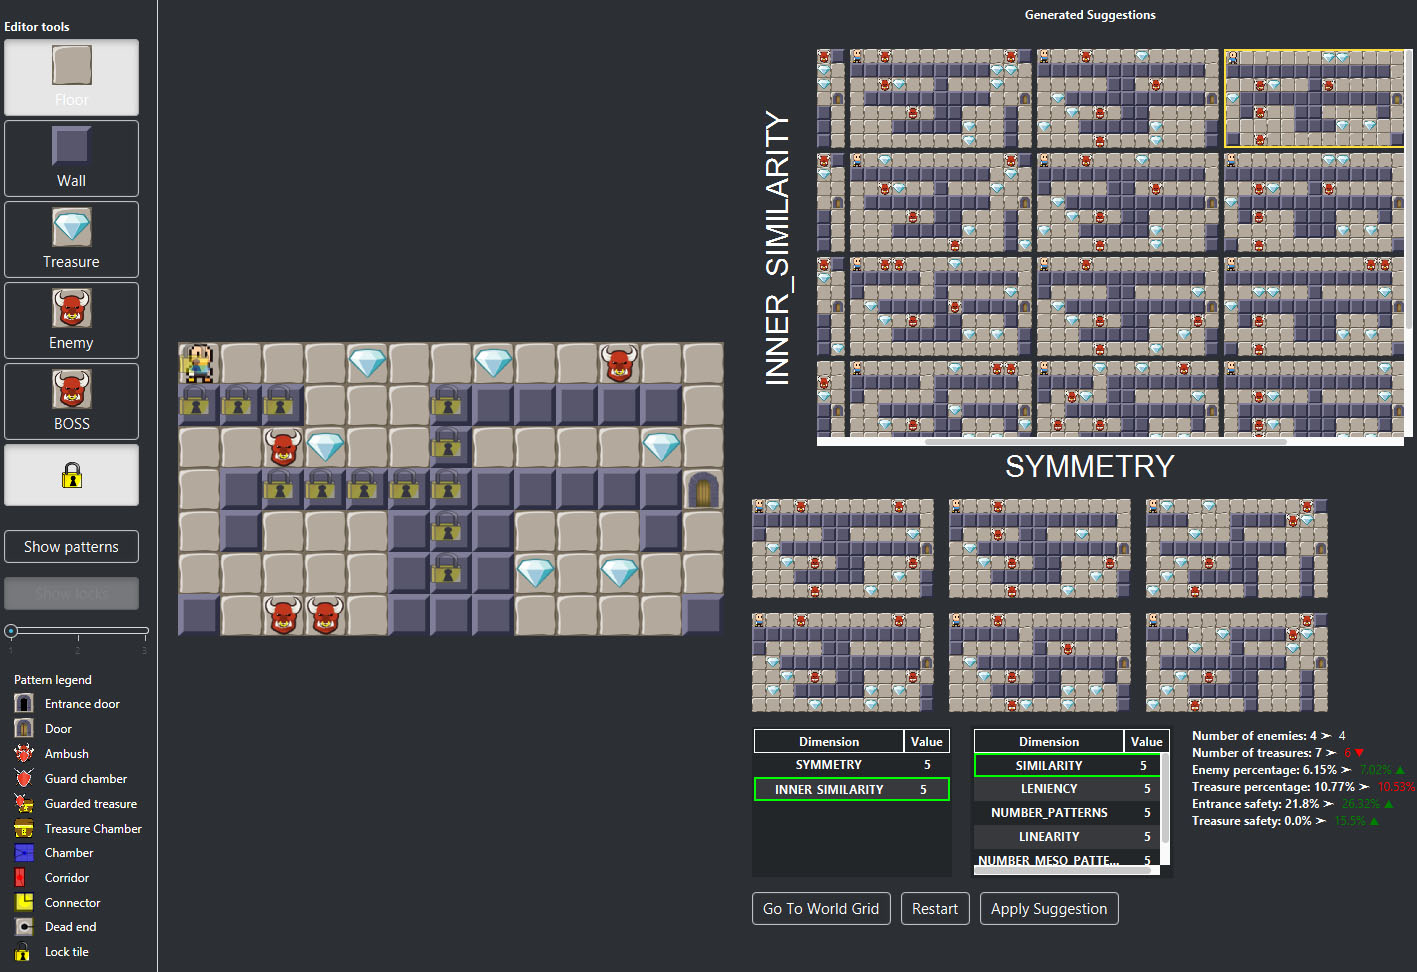
\includegraphics[width=9cm]{figures/figure1.png}}
% \caption{The main components in EDD. (a) A basic room, (b) different placeable tiles, (c) micro-patterns and (d) meso-patterns~\cite{p6Alvarez2018a}.}
% \label{figs:basecomponents}
% \end{figure}
\subsection{Background}

% Machine Learning (ML) has gained an increased interest from game researchers, achieving remarkable success on training AI agents for very popular games, such as AlphaStar on Starcraft 2 \citepsixth{p6alphastarblog} and OpenAI Five on Dota 2 \citepsixth{p6berner2019dota}. Its combination with PCG has led to the raise of  Procedural Content Generation via Machine Learning (PCGML), defined as the generation of game content by models that have been trained on existing game content \citepsixth{p6summerville2018procedural}, with applications to autonomous content generation, content repair, content critique, data compression, and mixed-initiative design. 

Player modeling, the ability to recognize general socio-emotional
and cognitive/behavioral patterns in players \citepsixth{p6thawonmas2019artificial}, has been appointed by the game research community as an essential process in many aspects of game development, such as designing of new game features, driving marketing and profitability analyses, or as a means to improve PCG and game content adaptation. Player modeling frequently relies on data-driven and ML approaches to create such models out of several sorts of user-generated gameplay data \citepsixth{p6liapismodellingquality19,p6melhart2020feel,p6Drachen2009-playerModellingTombRaider,p6Holmgard2019-proceduralPersonas,p6Melhart2019-ModellingMotivation}.

Using player data from \textit{Iconoscope}, a freeform creation game for visually depicting semantic concepts, Liapis et al. trained and compared several ML algorithms by their ability to predict the appeal of an icon from its visual appearance~\citepsixth{p6liapismodellingquality19}. Furthermore, Alvarez and Vozaru explored personality-driven agents based on individuals' personalities using the \textit{cibernetic big five model}, evaluating how observers judged and perceived agents using data from their personality test when encountering multiple situations~\citepsixth{p6Alvoz2019-PersonalityDriven}. 

%  using Bartle's player archetypes~\citepsixth{p6bartle1996-taxonomy}

Moreover, training models on gameplay data from \textit{Tom Clancy's The Division} has also been used to model, and therefore find predictors of player motivation \citepsixth{p6Melhart2019-ModellingMotivation}, which renders a very valuable tool for understanding the psychological effects of gameplay. Former research followed a similar approach in \textit{Tomb Raider Underworld}, training player models on high-level playing behavior data, identifying four types of players as behavior clusters, which provide relevant information for game testing and mechanic design \citepsixth{p6Drachen2009-playerModellingTombRaider}. Melhart et al. take these approaches one step further by modeling a user's \textit{Theory of Mind} in a human-game agent scenario \citepsixth{p6melhart2020feel}, finding that players' perception of an agent's frustration is more a cognitive process than an affective response. %Alvarez and Vozaru did similar work, exploring personality-driven agents based on individuals' personality using the \textit{cibernetic big five model}, evaluating how observers judged and perceived agents using data from their personality test when encountering multiple situations~\citepsixth{p6Alvoz2019-PersonalityDriven}.

%Alvarez and Vozaru did similar work, exploring personality-driven agents based on individuals' personality using the \textit{cibernetic big five model}, which treats personality-driven agents as goal-based entitites, evaluating how observers judged and perceived agents using data from their personality test when encountering multiple situations~\citepsixth{p6Alvoz2019-PersonalityDriven}.
%modeling individual agents based 

\subsubsection{The Player is the Designer}

Mixed-initiative co-creativity (MI-CC)~\citepsixth{p6yannakakis2014micc}, is the subset of PCG algorithms where human users and AI systems engage in a constant mutual inspiration loop towards the creation of game content \citepsixth{p6charity2020baba,p6machado2019pitako,p6shaker2013ropossum,p6smith_tanagra:_2011,p6liapis_generating_2013}. Understanding player behavior and experience, as well as predicting the player's motivation and intention is key for mixed-initiative creative tools while aiming to offer in real-time user-tailored procedurally generated content. Nevertheless, the player is the designer in MI-CC, and gameplay data is replaced by a compilation of designer-user actions and AI model reactions over time while both user and model are engaged in a mutually inspired creative process. A fluent MI-CC loop should provide good human understanding and interpretation of the system, as well as accurate user behavior modelling by the system, capable of projecting the user's subsequent design decisions \citepsixth{p6ComptonPhD}. 

%Similar to user or player modeling, designer modeling for content creation tools (CAD and MI-CC tools) was suggested by Liapis et al~\citepsixth{p6Liapis2013-designerModel}, where it is proposed the use of designers models that capture their styles, preferences, goals, intentions, and interaction processes. In their work, they suggest methods, indications, and advice on how each part can be model to be integrated into a holistic designer model, and how each game facet can use and benefit from designer modeling. Moreover, in \citepsixth{p6Liapis2014-designerModelImpl} the same authors discuss their implementation of designer modeling and the challenges of integrating all together in their MI-CC tool, Sentient Sketchbook, which had a positive outcome on the adaptation of the tool towards individual “artificial” users.

Shifting towards a designer-centric perspective means that besides focusing on player modeling, it is necessary to focus on modeling the designers. Liapis et al.~\citepsixth{p6Liapis2013-designerModel,p6Liapis2014-designerModelImpl} introduced designer modeling for personalized experiences when using computer-aided design tools, with a focus on the integration of such in automatized and mixed-initiative content creation. The focus is on capturing the designer's style, preferences, goals, intentions, and iterative design process to create representative models of designers. Through these models, designer's and their design process could be understood in-depth, enabling adaptive experiences, further reducing their workload and fostering their creativity. 

%\citepsixth{p6charity2020baba,machado2019pitako,shaker2013ropossum,smith_tanagra:_2011,Machado2017,liapis_generating_2013}. 

% Moreover, goal 13 in the guidelines for Human-AI interaction \citepsixth{p6amershi2019guidelines} highlights the importance of learning from user behavior and personalize the user’s experience by learning from their actions over time. 


%Nourani et al.~\citepsixth{p6Nourani2019-meaningfulExplanations}, who discuss the effects of meaningful and meaningless explanations to users of an AI interactive systems, and their results demonstrates that when an explanation is not aligned with human-logic it significantly affect the user's perception of the system and it's usability is hindered.

Furthermore, lack of transparency is a key impediment for the advancement of human-AI systems, being eXplainable AI (XAI) an emergent research field that holds substantial promise for improving model explainability while maintaining high-performance levels~\citepsixth{p6adadi2018peeking,Doshi-Velez2018}. However, explanations should be aligned with the users' understanding to don't hinder the usability of systems, as demonstrated by Nourani et al.~\citepsixth{p6Nourani2019-meaningfulExplanations}, who discuss the effects of meaningful and meaningless explanations to users of an AI interactive systems.

Zhu et al.~\citepsixth{p6Zhu2018-XAIDesignersMICC} proposed the field of eXplainable AI for Designers (XAID) as a human-centered perspective on MI-CC tools. This work discusses three principles of mixed-initiative, \emph{explainability}, \emph{initiative}, and \emph{domain overlap}, where the latter focuses on the study of the overlapping creative tasks between game designers and black-box PCG systems in mixed-initiative contexts. This work deems of high relevance the inclusion of data-driven and trained artifacts to facilitate a fluent bi-directional communication of the internal mechanisms of such a complex co-creative process in which \textit{the designer provides the vision, the AI provides capabilities, and they merge that into the creation}. Mapping the designer's internal model to the AI's internal model is suggested as a meaningful way for creating a common ground that establishes a shared language that enables such communication. In the same line, Xie et al.~\citepsixth{p6xie2019interactive} explored visualization techniques through an interactive level designer tool called \textit{QUBE} to explain and introduce machine learning principles to game designers.

Moreover, Guzdial et al.~\citepsixth{p6guzdial-lvldsg-aiide-2018} discuss the insufficiency of current approaches to PCGML for MI-CC, as well as the need for training on specific datasets of co-creative level design. Guzdial et al. work on the mixed-initiative Morai Maker~\citepsixth{p6guzdial2019friend} shows the relevance of exploring the ways designers and AI interact towards co-creation, identifying four human-AI relationships (friend, collaborator, student, and manager), as well as the different ways they impact on the designer-user experience. Our study advocates for the importance of designer modeling through ML as the generation of surrogate models of designer styles by training on existing designer-generated data, aiming for an improvement in quality and diversity in computational creativity and, in particular, MI-CC tools. 

\subsubsection{The Designer Preference Model in EDD}

EDD is an MI-CC tool where designers can create dungeons and rooms; meanwhile, a PCG system analyzes their design and proposes generated suggestions to the designer~\citepsixth{p6Alvarez2018, Baldwin2017}. EDD uses the \emph{Interactive Constrained MAP-Elites} (IC-MAP-Elites)~\citepsixth{p6alvarez2019empowering}, an evolutionary algorithm that combines Constrained MAP-Elites~\citepsixth{p6Khalifa2018} with interactive and continuous evolution. 

The work presented in \citepsixth{p6Alvarez2020-DesignerPreference} introduced the Designer Preference Model, a data-driven solution that learns from user-generated data in the MI-CC Evolutionary Dungeon Designer. This preference model uses an Artificial Neural Network to model the designer based on the choices she makes while using EDD. Both systems constantly interact and depend on each other, so that the Designer Preference Model learns from the generated and selected elites, and IC-MAP-Elites uses the Designer Preference Model as a surrogate model of the designer to complement the fitness evaluation of new individuals. 

This approach's main goal is modeling the user's design style to better assess the tool's procedurally generated content, increasing the user's agency over the generated content without stalling the MI-CC loop \citepsixth{p6ComptonPhD} or increasing user fatigue with periodical suggestion handpicking \citepsixth{p6liapis2016mixed,p6Takagi2001-InteractiveEvo}. The results showed the need for stability and robustness in the data-driven model, to counterbalance the highly dynamic designer's creative process. 


\subsection{Room Style Clustering}

% \begin{enumerate}
%     \item Information on the user studies and how we develop the clusters.
%     \item collected data through 2 user studies
%     \item transformed the data into 5 datasets
%     \item data reduction through PCA and T-SNE. Cluster with K-means, K-Medoids, agglomerative clustering and DBSCAN. Evalulated through internal indices (silhouette index, DB index, and CH-index) 
% \end{enumerate}

\begin{figure*}[ht!]
\centerline{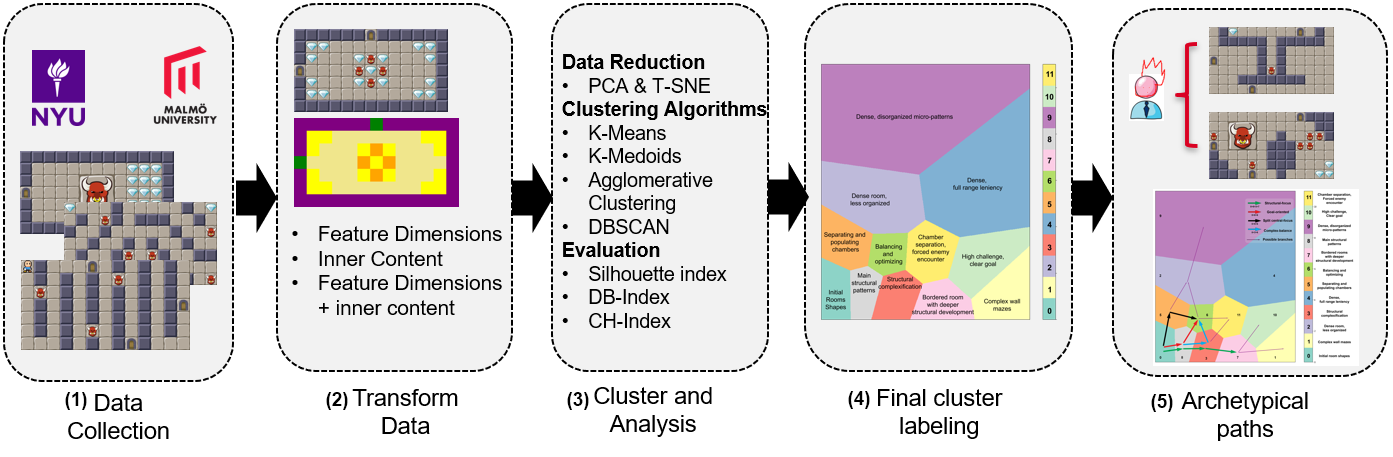
\includegraphics[width=\textwidth]{figures/process-steps.png}}
\caption{The stages of the design style clustering development: (1) Data was first collected through two user studies. (2) Then, using the design sequences, the data was processed into five different datasets, one using the room images, a second using the tiles information, and three using tabular information. (3) A data reduction technique was applied to different datasets, and then they were clustered and internally evaluated. (4) The clusters were formed, picked from the best performing methods, and labeled based on the data points within each cluster. The cluster were evaluated by visualizing how a typical design session traverse the various clusters, and K-Means (K=12) was chosen as the final approach. (5) Finally, using this final approach all the sequences were clustered and archetypical paths were identified.%(5) The final approach,  K-Means (K=12) was evaluated by visualizing how a typical design session traverse the various clusters. Finally, the sequences were clustered by the final approach and archetypical paths were identified.
} \label{p6fig:approach-steps}
\end{figure*}

\begin{figure*}[t]
\centerline{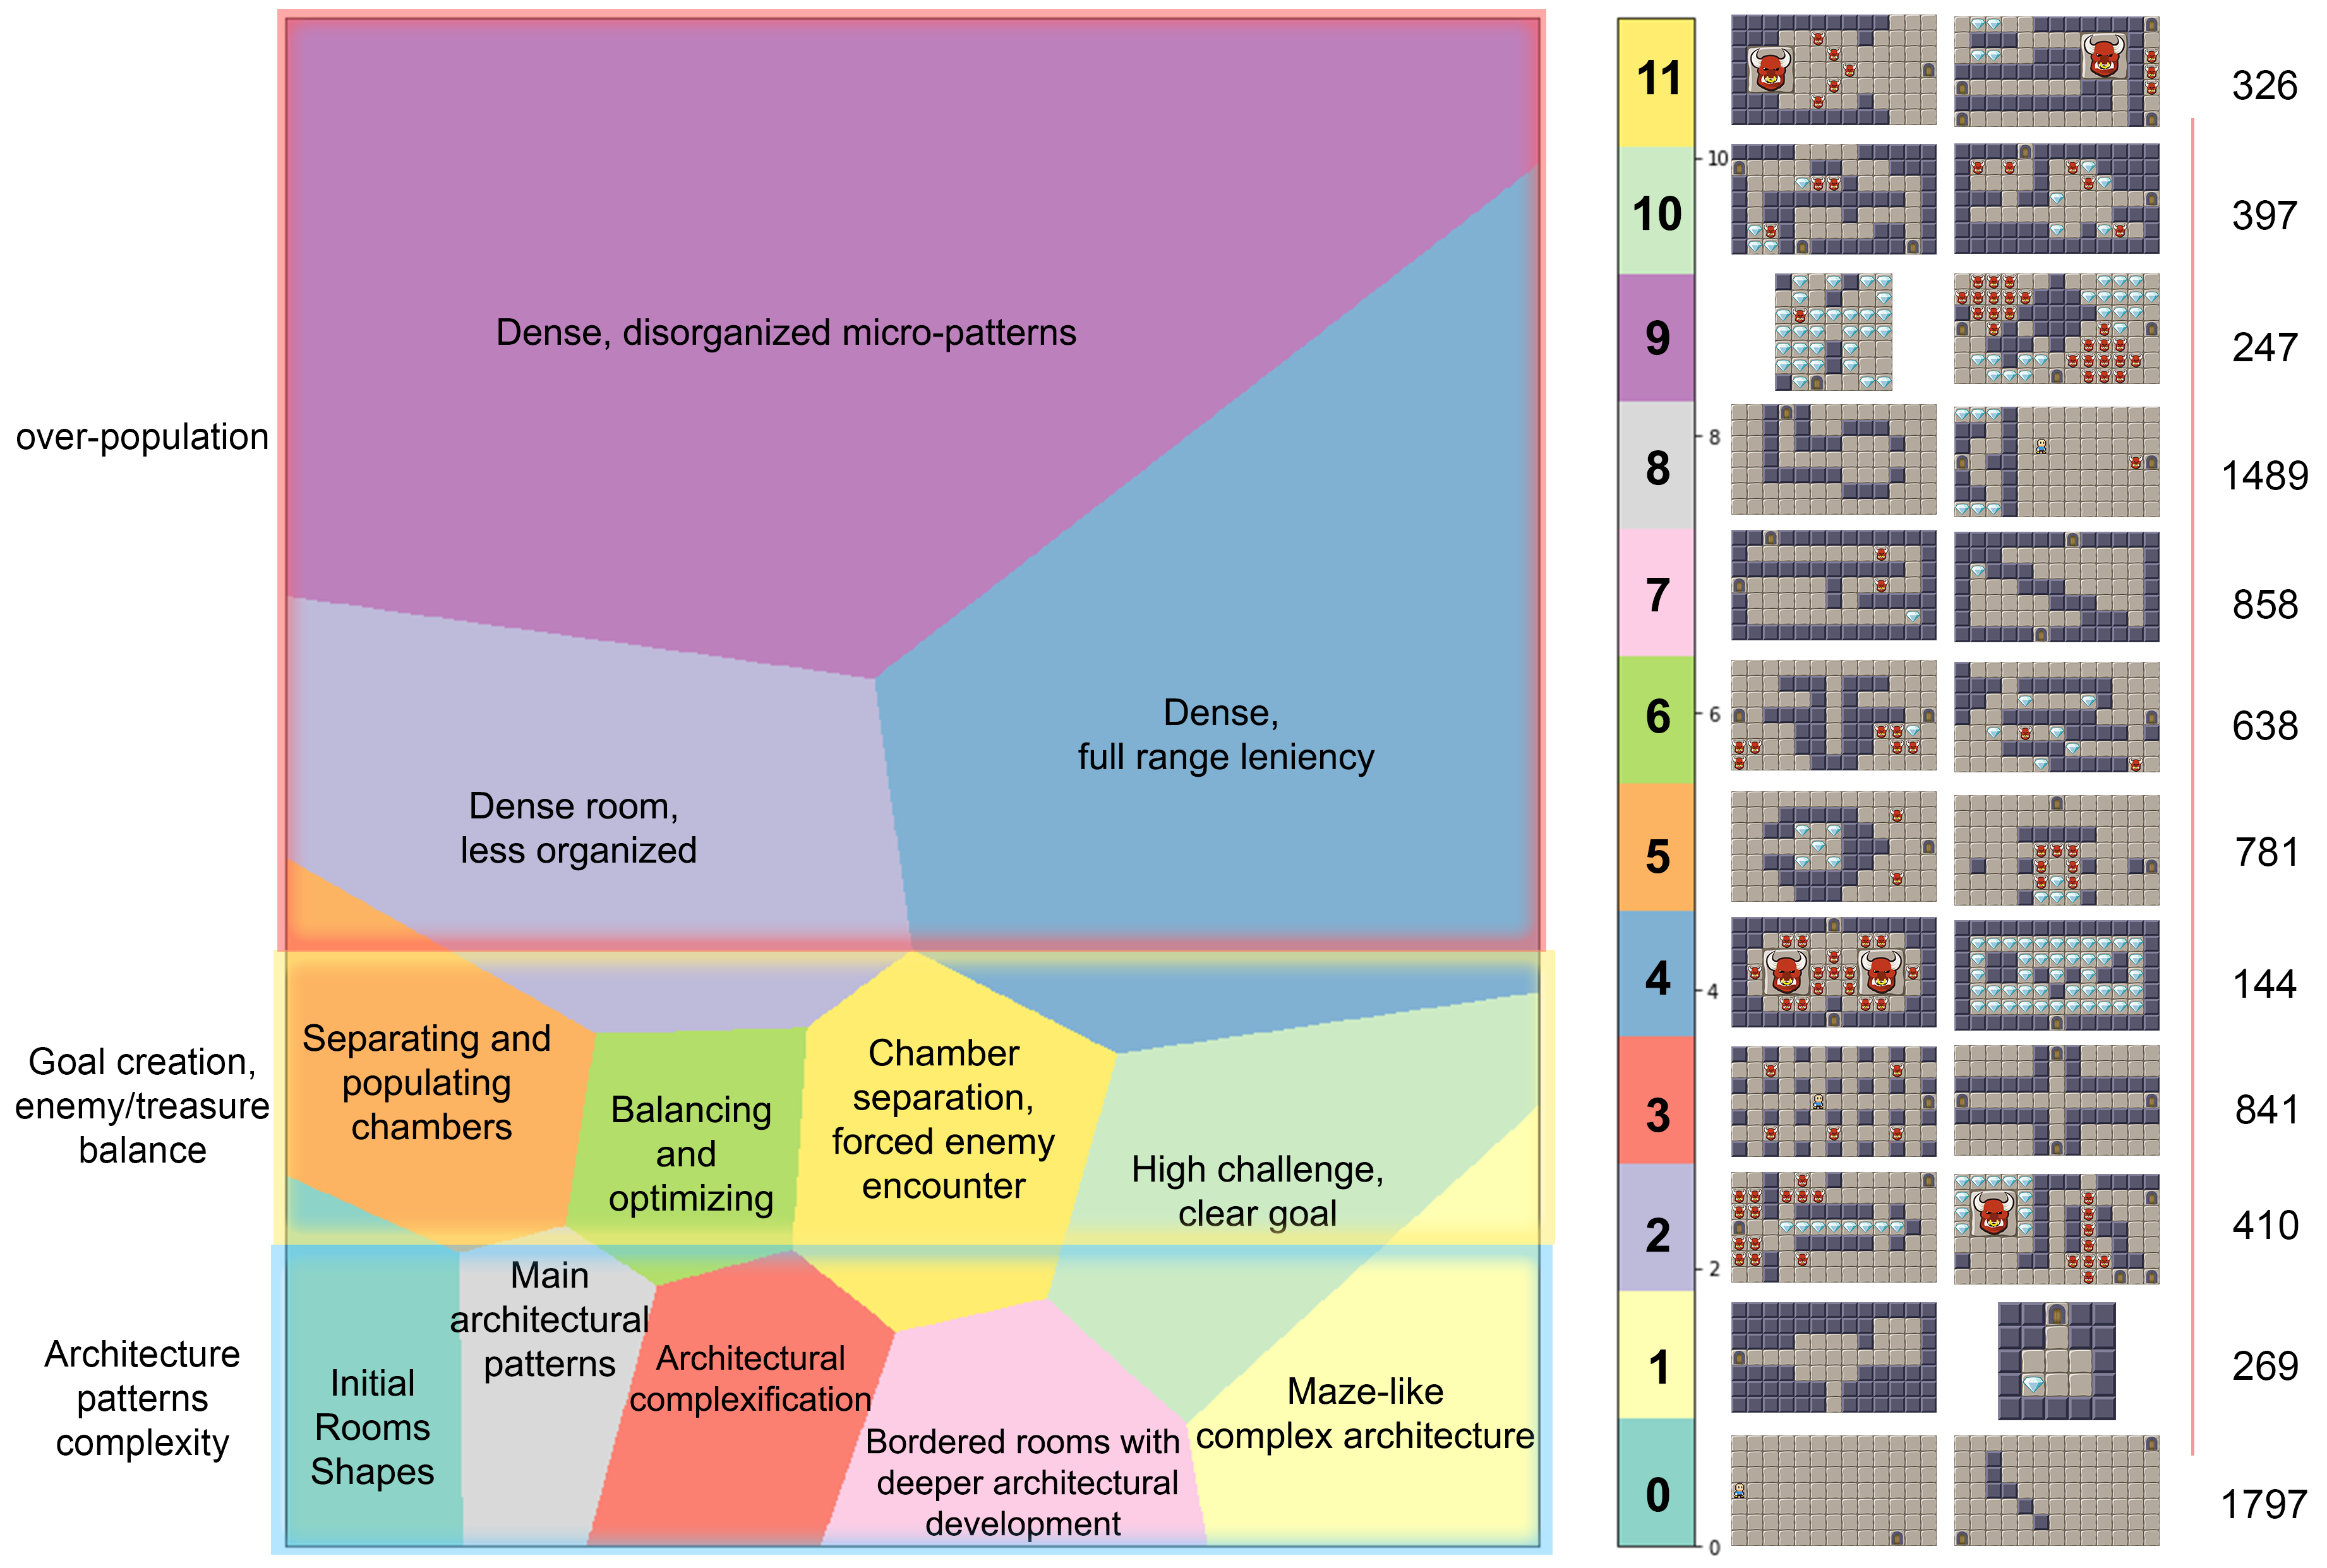
\includegraphics[width=\textwidth]{figures/final-cluster.png}}
\caption{Best resulting cluster set. K-Means (K=12), using the \textbf{Tiles} Dataset. While it scores slightly less in the internal indices that other setups, a qualitative analysis successfully gives us more granularity by subdividing the main bottom clusters, to label and cluster the design process of designers. Sample rooms belonging to each cluster are displayed on the right, next to the total number of rooms in the cluster.} \label{p6fig:all-clusters}
\end{figure*}

% \begin{figure*}[b]
% \centerline{\includegraphics[width=13cm]{figures/representative cluster-steps.png}}
% \caption{Examples of a step by step edition sequence of a design session and it's clustering. To the left, we present the actual sequence and steps of one of the rooms in the dataset and to the right is the actual trajectory of the design in the cluster space. Numbered and in black, it is shown how each step of the design process is clustered by our approach} \label{p6fig:paths-designers}
% \end{figure*}

% \begin{figure}[h]
% \centerline{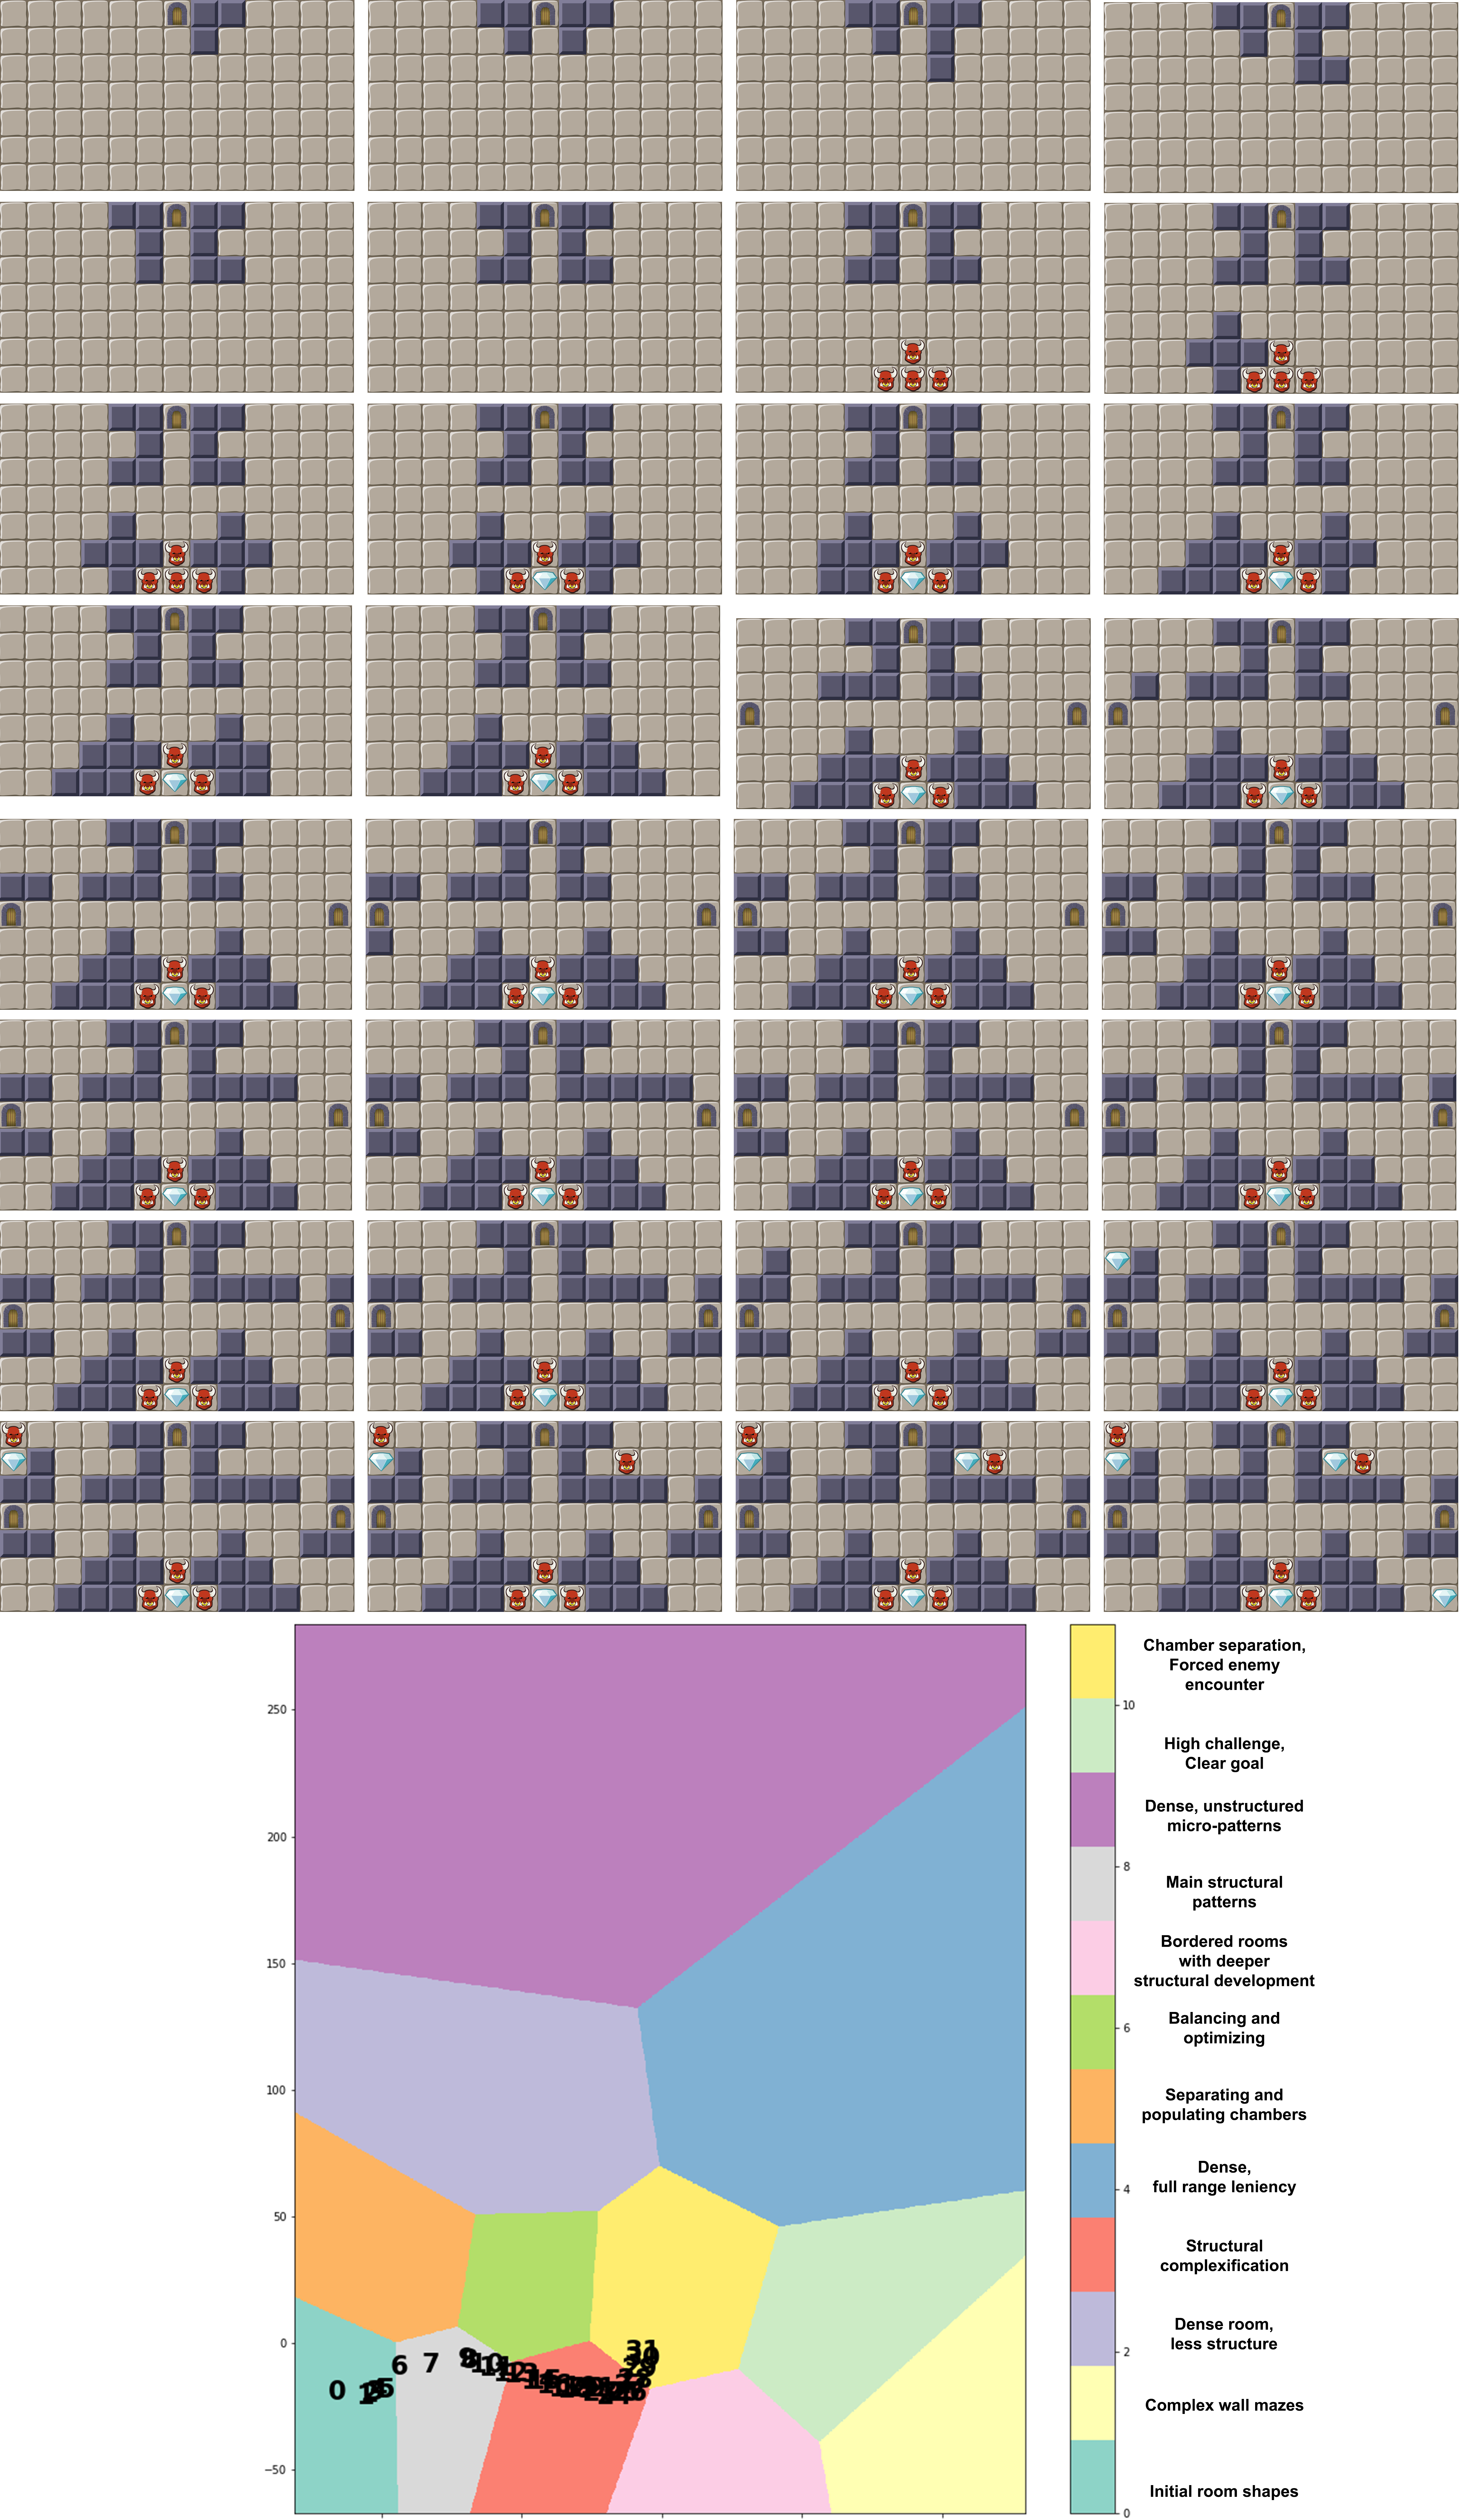
\includegraphics[width=8cm]{figures/representative-cluster-steps-alter.png}}
% \caption{Example of a step by step edition sequence of a design session and it's clustering. At the top, we present the actual sequence and steps of one of the rooms in the dataset, in a $4\times7$ grid, starting at the top left with the first edition. At the bottom, it is the actual trajectory of the design in the cluster space. Numbered and in black, it is shown how each step of the design process is clustered by our approach} \label{p6fig:paths-designers}
% \end{figure}

\begin{figure*}
\centerline{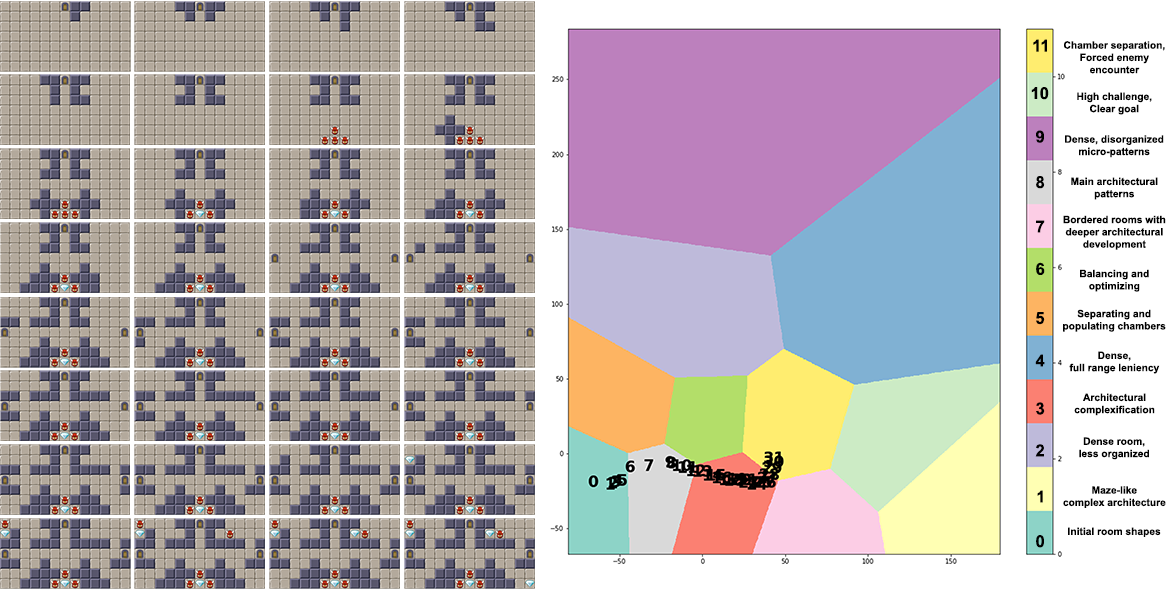
\includegraphics[width=\textwidth]{figures/representative-clusters-small.png}}
\caption{Example of a step by step edition sequence of a design session and it's clustering. At the left, we present the actual sequence and steps of one of the rooms in the dataset, in a $4\times7$ grid, starting at the top left with the first edition. At the bottom, it is the actual trajectory of the design in the cluster space. Numbered and in black, it is shown how each step of the design process is clustered by our approach} \label{p6fig:paths-designers}
\end{figure*}

This paper presents an approach and fundamental steps towards the implementation of designer personas: an analysis of designer style clustering to isolate archetypical paths that can be later be used to build ML surrogate models of archetypal designers. Such models would adapt to the dynamic designer during the mixed-initiative creative process by being placed in the solution space, allowing the designer to traverse such space of models as she drifts through the many dimensions of her creative process.

The proposed system builds on top of EDD's Designer Preference Model and preliminary results \citepsixth{p6Alvarez2020-DesignerPreference}, expanding it to classify the designers' designs based on clusters developed using previously hand-made design sequences by expert and non-expert designers. Figure \ref{p6fig:approach-steps} illustrates our approach in five sequential stages, from data collection to experimentation and results. The first four stages are explained in the following subsections, whereas Section~\ref{p6section:results} shows the experimental results.

\subsubsection{Data Collection}

We conducted two user studies where participants were tasked with freely designing a dungeon in EDD and the rooms that compose it with no further restrictions, using all the available tiles i.e. floor, wall, treasure, enemy, and boss tiles. All participants were introduced to the tool before the design exercise. User-generated data was gathered during the complete design session, creating a new data entry every time the designer edited the dungeon. In total, we had $40$ participants, $25$ of these (i.e. NYU participants) were industry or academic researchers within the Games and AI field, and the other $15$ (i.e. MAU participants) were game design students. This resulted in a diverse dataset composed of $180$ unique rooms like the ones depicted in Figure~\ref{p6fig:approach-steps}, that was pre-processed and clustered in the subsequent stages. 

\subsubsection{Dataset pre-processing}

From the $180$ unique rooms, we extracted and used the edition sequence of each of the rooms, from their initial design to the more elaborated end-design, to compose a richer dataset that could capture the design process of a designer rather than focusing on the end-point. Through this, we ended up using $8196$ data points in our dataset.
%just the end-point. We ended up using $8196$ rooms
Moreover, five different copies of the dataset were created to analyze and compare the performance of the clustering stage using the following image pre-processing methods:

\begin{enumerate}
\setcounter{enumi}{0}
    \item \textbf{Room:} No pre-processing. Room images are fed into the next stage as they were created by the designer, with a resolution of $1300\times 700\times3$, corresponding to width, height, and RGB ($3$ color channels).
    
    \item \textbf{Tiles:} Each room tile type is mapped to a single-color pixel and the rooms are simplified to a pixel-tile based representation, as shown in the second stage of Figure \ref{p6fig:approach-steps}. The dimensions are downscaled to $13\times 7\times3$.
    %Each room tile is simplified to a single-color pixel, as shown in the second stage of Figure \ref{p6fig:approach-steps}, downscaled to $13\times 7\times3$.
    
    \item \textbf{Dimensions:} Each room is described by its five IC-MAP-Elites feature dimension values, excluding the similarity scores: \textsc{Linearity}, \textsc{Leniency}, \textsc{\#MesoPatterns}, \textsc{\#SpatialPatterns}, and \textsc{Symmetry}. A complete description of these features can be found in~\citepsixth{p6Alvarez2020-ICMAPE}.
    
    \item \textbf{Inner Content:} Each room is described by $12$ values, related to the count, sparsity, and density of the enemy, treasure, floor, and wall tiles contained in it.
    
    \item \textbf{Combined:} A combination of the \textbf{Dimensions} and \textbf{Inner Content} methods.
\end{enumerate}

\subsubsection{Clustering and Analysis}

To run all setups, data reduction algorithms, clustering algorithms, and do the internal evaluation of the clusters, we used scikit-learn machine learning toolset~\citepsixth{p6scikit-learn}. To obtain the best set of clusters, we ran different setups with the above datasets. The data was reduced to two meaningful dimensions with two different data reduction algorithms, Principal Component Analysis (PCA) and T-Distributed Stochastic Neighbor Embedding (T-SNE). For both data reduction algorithms, we fit the algorithms with each individual dataset, setting to two principal components and in the case of T-SNE using PCA as initializing algorithm, and transforming the data into a new dataset \emph{pca\_dataset} and \emph{tsne\_dataset} per dataset. Each two-dimensional point in the new datasets represents a step in the sequences described above.%Likewise, for the T-SNE, we fit the algorithm with each individual dataset, setting the parameters to two principal components and using PCA as initializing algorithm, and then transformed the data into a new dataset \textit{tsne_dataset} per dataset.

Moreover, all the resulting datasets were then clustered using \textsc{K-Means, K-Medoids, Agglomerative clustering}, and \textsc{DBSCAN}. K-Means was initialized using the standard k-means++ implemented in scikit-learn, which initialize all centroids distant from each other. K-Medoids was initialized similarly, using the standard k-medoids++, and tested using the \emph{cosine}, \emph{euclidean}, and \emph{manhattan} distances. Agglomerative clustering is a hierarchical clustering approach using a bottom-up approach implemented in scikit-learn using four different linkage criteria for comparing data points: \emph{Ward}, \emph{Complete}, \emph{Average}, and \emph{Single}. Finally, DBSCAN cluster points based on density separated by low-density areas; thus, DBSCAN automatically finds $k$ based on two parameters, $\epsilon$ describing the maximum distance between points and \emph{min\_samples} describing the minimum amount of samples within a group to be considered a cluster. K-Means, K-Medoids, and Agglomerative clustering were tested using multiple $K$ values ranging from 3 to 13, and DBSCAN was tested with several $\epsilon$ values ranging from 0.3 to 1.0, and \emph{min\_samples} ranging from 2 to 9.

%, testing with $K$ values ranging from 3 to 13 for the first three ones, and several $\epsilon$ values for DBSCAN.

%testing different minimum distance between data points ($\epsilon$) and the minimum amount of data points within a cluster to be considered a dense region for DBSCAN.

Since we lack a labeled dataset (i.e. ground truth) for cluster validation, we evaluated the results from all setups using the internal indices below, as well as manually inspecting the rooms composing the resulting clusters.

%Since in our approach lacks a labeled dataset (i.e. ground truth) for cluster validation, 

\begin{itemize}
\item \textbf{Silhouette Score:} The Silhouette Score shows how similar a data point is to the cluster it is associated with, through calculating the difference between the $\overline{distance}$ from the point to the points in the nearest cluster and the $\overline{distance}$ to the points in the actual cluster. The value is bounded from -1 to +1, with values closer to +1 indicating a good separation of the clusters, and closer to -1 meaning that some points might belong to another cluster.
\item \textbf{Davies-Bouldin Index:} The DB-index is the ratio between the within-cluster distances and between-clusters distances. With this, we can have an insight into the average similarity of clusters with their closest cluster. The value is bounded from 0 to +1, with values closer to 0 relate to clusters that are farther apart from each other and less dispersed, thus, this index is more crucial when we have more dense representations.
\item \textbf{Calinski-Harabasz Index:} The CH-index is another index related to the density of the clusters and how well separated they are. The score is the ratio between the within-cluster dispersion (compactness) and the between-cluster dispersion (separation). The CH-index is positively unbounded, and the higher the score the better.
\end{itemize}

\subsubsection{Cluster Labelling}

\begin{table}
\begin{center}
{\caption{Best performing setups based on their internal validation and visualization of clustered data points.}\label{p6table:setups}}
\resizebox{0.9\textwidth}{!}{
\begin{tabular}{ccccccc}
\hline
\rule{0pt}{12pt}
Algorithm&Data&K&$\Diamond$&$\Box$&$\bigtriangleup$ 
\\ 
\hline
\\[-6pt]
K-Means & Tiles-PCA & 9 & 0.43 & 0.73 & 9438.233 \\ 
K-Means & Tiles-PCA & 12 & 0.41 & 0.77 & 9436.928 \\
K-Means & Dimensions-PCA & 12 & 0.43 & 0.73 & 7738.343 \\
Agglomerative single & Combined-PCA & 6 & 0.51 & 0.43  & 38.833 \\ 
Agglomerative avg. & Dimensions-PCA & 6 & 0.44 & 0.67 & 3463.567 \\ 
\hline
\\[-6pt]
\multicolumn{6}{l}{$\Diamond$ Silhouette Score\ \
$\Box$ Davies Bouldin Index\ \
$\bigtriangleup$ Calinski-Harabasz Index}
\end{tabular}
}\end{center}
\end{table}

Table~\ref{p6table:setups} shows the best performing setups according to their internal indices scores. The clusters in these setups were manually inspected in order to detect the qualitative features that better define them. 

When using the \textbf{Dimensions} and \textbf{Combined} datasets, the clusters do perform good, if not better, in certain indices than when using the \textbf{Tiles} dataset. However, when analysing the resulting setups, they were missing a clearer relation between the clustered rooms, which was exacerbated when analysing sequences and paths on these setups, where they missed continuity between clusters.

Conversely, given that we are creating tile-based rooms and dungeons, the features were more representative for the \textbf{Tiles} dataset, which when used, generally performed well in the evaluated internal indices, and the produced clusters meaningfully separate the data. Further, as it will be presented in Section \ref{p6section:results}, when clustering sequences and analyzing the cluster path of the designs, there exist a continuity between designs that supports its usability. Figure \ref{p6fig:all-clusters} shows the best-resulting cluster set found among all the experiments run.



% As expected, the \textbf{Tiles} dataset generally performed well in the evaluated internal indices, and the produced clusters meaningfully separated the data.
% better information and were meaningfully group together.  relation each of the features have with 

% As expected, the \textbf{Tiles} representation have good results across the 3 indices, 

% JOSÉ: I leave it here waiting for the final results from Alberto

%Moreover, We noticed that the agglomerative approach results in very specific clusters alongside a quite broad cluster consisting of unrelated data points, regardless of the $K$ used. These setups scored well in the different indices but fail to accurately partition the space in relevant groups.

%Moreover, there are recurrent clusters between the different setups but when using more clusters like in figure~\ref{p6fig:all-clusters} (b), we can have more granularity when partitioning the space, improving the separation of more related data points. In figure~\ref{p6fig:all-clusters}(b) we present several rooms that have been clustered together matching the labeling of the clusters. In the figure, there is a clear correlation between the designs and the labels of their respective cluster, and an interesting continuity between the final clusters.

% In Figure~\ref{p6fig:all-clusters}, we present the final and selected approach for clustering room styles using K-Means (K=12) and the \textbf{Tiles} dataset reduced with the PCA algorithm. To the right, next to each color in the legend, we have different representative rooms that belong to the clusters, in their respective color, and have been clustered together. Furthermore, besides the local relation between clusters, there exists a layered division among group of clusters in the y-axis, where the bottom clusters relate more to architectural pattern complexity, from very empty rooms to mazes. The middle clusters focus on populating the rooms with enemies and treasures, creating the actual goals of the room and balancing the challenge. Finally, the top clusters are composed of dense rooms where the enemy and treasure addition do not necessarily need to follow any clear objective. 


% The clusters's label are plotted on top of each of the clusters, describing in general, the content that is within them. These cluster 

In the figure, we have plotted on top of the clusters the labels describing in general, the content that is within them. The following is a description of the clusters and the rooms that were clustered together:

\textbf{0. Empty-Initial rooms:} %This cluster contains $1797$ data points, and 
This cluster relates mostly to the initial designs made by the designers. These designs are from completely empty rooms to initial work-in-progress structures.

\textbf{1. Maze-like complex architecture:} This cluster to the extreme of the architectural patterns complexity layer, relates to more highly-linear, confined and maze-like rooms.% with more structure on what is possible. %The cluster contains $269$ data points.

\textbf{2. Dense, less organized:} This cluster contains rooms that still have a certain objective but are moving towards more disorganized distributions of micro-patterns in relation to their density. %This cluster contains $410$ data points.

\textbf{3. architectural complexification:} %This cluster contains $841$ data points, and 
This cluster relates mostly to the complexification of wall structures by having dense wall chunks, representative architectural patterns, or symmetrical patterns.

\textbf{4. Dense, full range leniency:} Focusing on density as the other two clusters within the same layer, this cluster relates to rooms that are in the full range of leniency from very rewarding, treasure rooms to very challenging boss rooms. %This cluster contains $144$ data points.

\textbf{5. Separating and populating chambers:} This cluster relates to the process of separating rooms into distinct chambers, focusing on the center of the room, and starting to populate rooms with enemies and treasures. %The cluster contains $781$ data points.

\textbf{6. Balancing and optimizing:} This cluster contains a mix between corridors and chambers within rooms with a focus on balancing rooms and optimizing their design towards certain goals. %The cluster contains $638$ data points.

\textbf{7. Bordered rooms with deeper architectural development:} This cluster relates mostly to rooms with an added wall border by the designer, and where the focus is to shape chambers and develop more visual structures.

\textbf{8. Main architectural shapes:} Similar to other clusters within the same layer, this cluster relates to the development and definition of main architectural patterns that are somewhat symmetric.

\textbf{9. Dense, disorganized micro-patterns:} This cluster clusters the extreme rooms that contain a high density of tiles, other than floor-tiles, without a clear structure or objective for the player.

\textbf{10. High challenge, clear goal:} This cluster relates to well-shaped rooms with clear wall structures and goals, towards more challenge. 

\textbf{11. Chamber separation with forced enemy encounter:} This cluster relates to rooms that are in the process of a clear segmentation into corridors and chambers, and that enforce to some extent, enemy encounters for the player. 

Furthermore, besides the local relation between clusters, the clusters are implicitly divided in three layers on the Y-axis. From bottom to top, (a) architectural patterns complexity, relating to clusters composed of rooms with clearer or complex shapes done with walls, from empty rooms to mazes. (b) Goal creation, enemy/treasure balance, with clusters comprehending the strategic addition of enemies and treasures to establish objectives in the room for the player. In terms of EDD, these rooms are composed of more meso patterns. And (c), over-population, which relates to clusters filled with less organized and dense rooms where the enemy and treasure addition do not necessarily need to follow any clear objective. Identifying the designer in such layer, and the path they have taken to get there could show meaningful information in the design process. For instance, the intentions of the designer, in what phase of the design process she is at the moment i.e. trying the tool or observing how the tool reacts or scraping her current goal towards a new goal within the room. 

% \begin{enumerate}
% \setcounter{enumi}{-1}
% \item[0] \textbf{Empty/Initial rooms:}
% \item \textbf{Complex wall mazes:} 
% \item \textbf{Dense, less structure} 
% \item \textbf{Structural complexification:} 
% \item \textbf{Dense, full range leniency} 
% \item \textbf{Separating and populating chambers:} 
% \item \textbf{Balancing and optimizing rooms:} 
% \item \textbf{Bordered rooms with deeper structural development:}
% \item \textbf{Development of main structural shapes:} 
% \item \textbf{Dense, unstructured:} 
% \item \textbf{Challenging rooms with clear goal:} 
% \item \textbf{Chamber separation with forced enemy encounter:} 
% \end{enumerate}



\begin{figure*}[t!]
\centerline{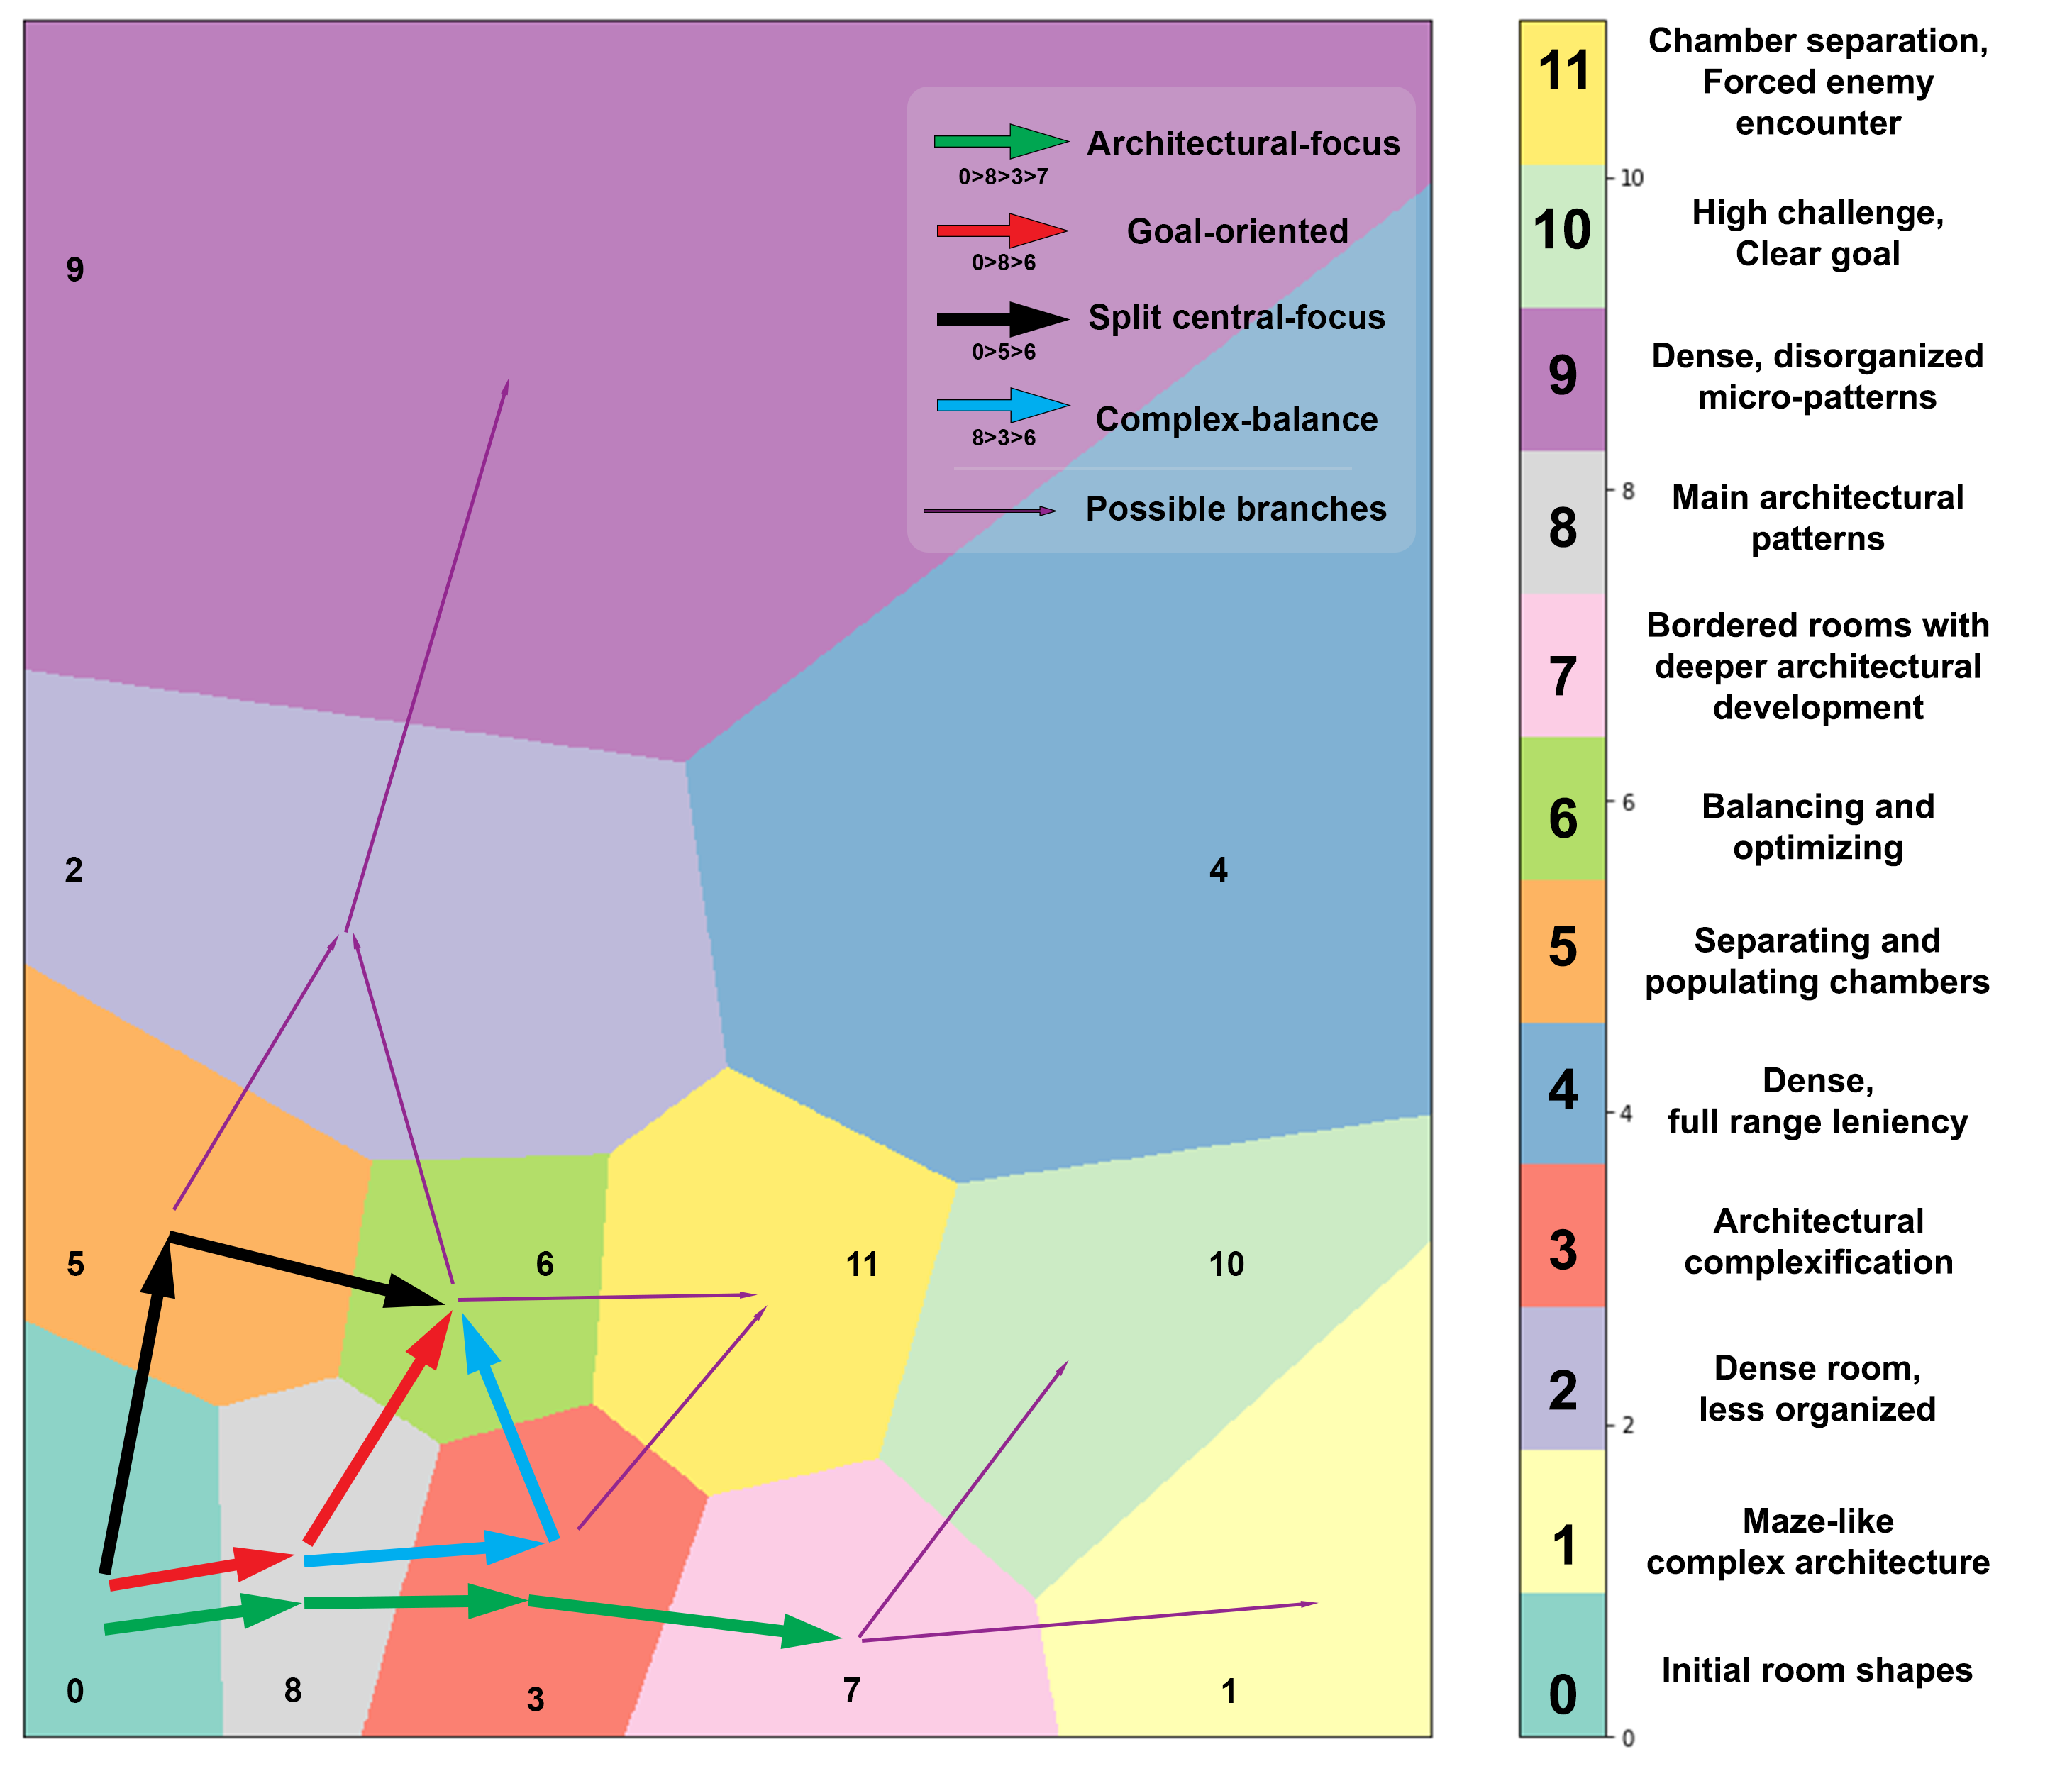
\includegraphics[width=\textwidth]{figures/resulting-paths-FINAL.png}}
\caption{Final and common designer trajectories. With thick arrows it is presented the archetypical paths, calculated using the frequencies of subsequences from $180$ diverse rooms. Each color represent a unique trajectory; with green the \textsc{Architectural-focus}, with red the \textsc{Goal-oriented}, with black the \textsc{Split central-focus}, and with blue the \textsc{Complex-balance}. Finally, thinner purple arrows extending from clusters traversed by the archetypical paths show the multiple possible branches that an archetypical path can deviate or extend to.} \label{p6fig:finalPaths}
\end{figure*}

% \begin{figure*}[t]
% \centerline{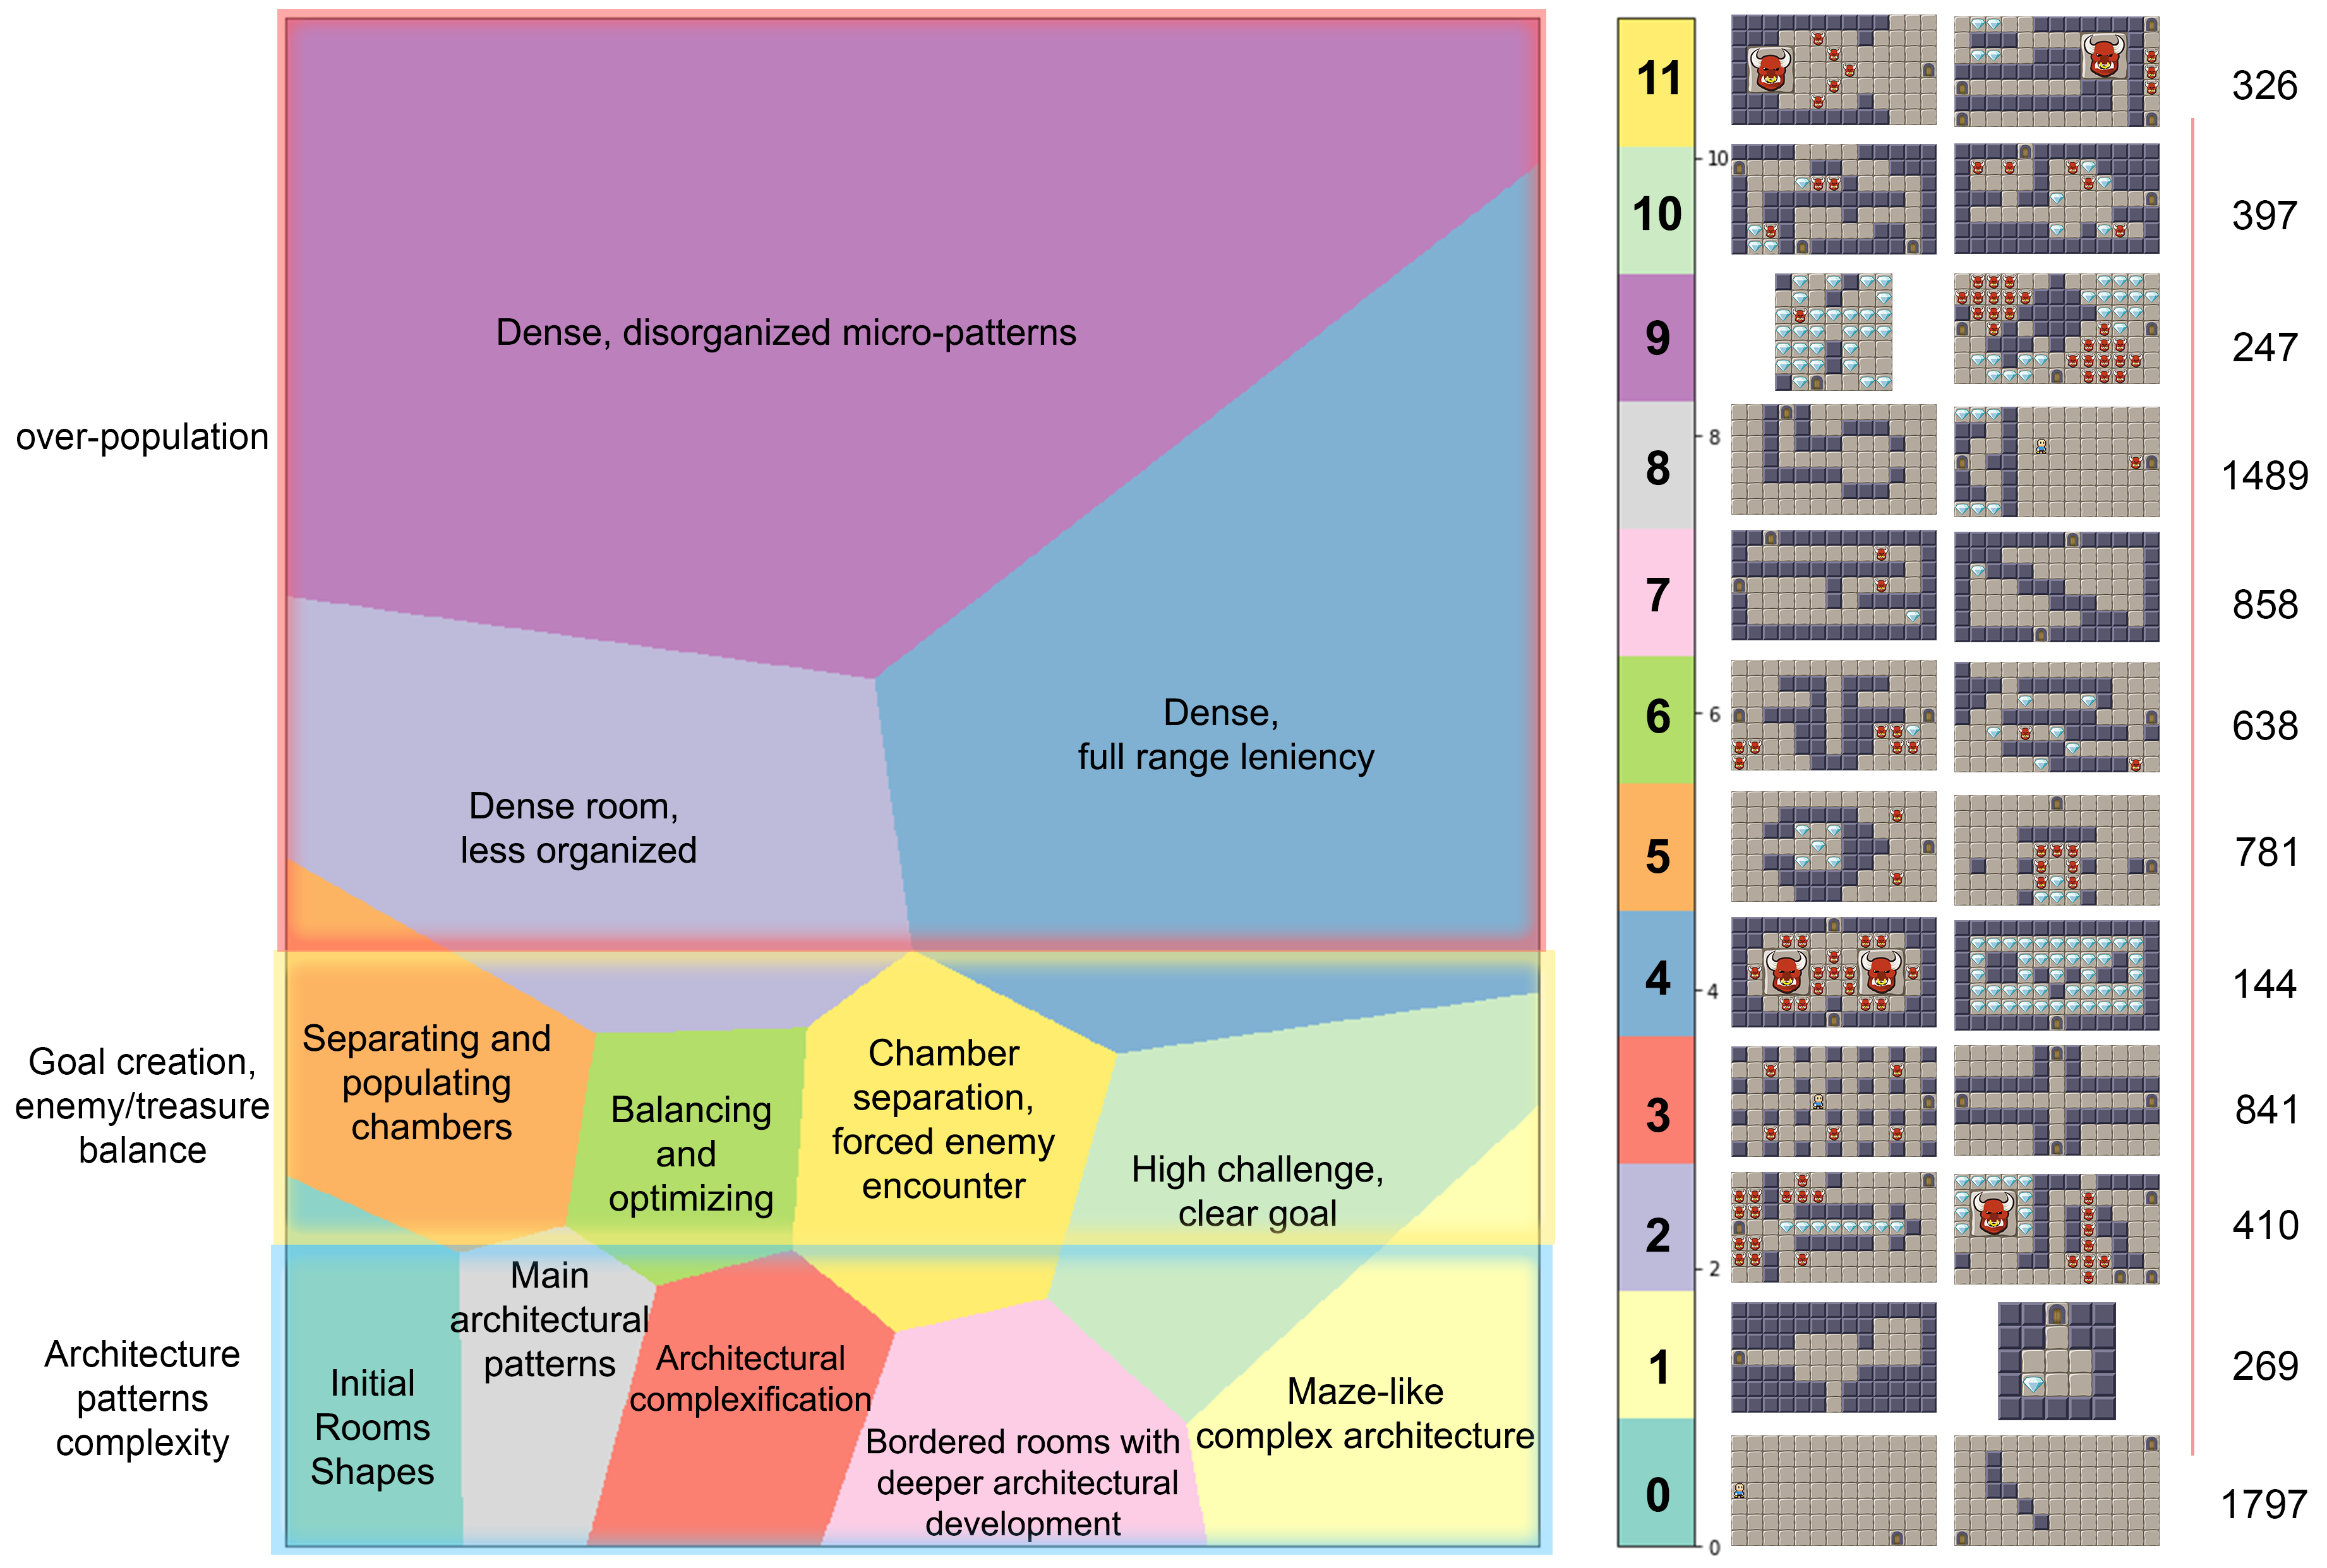
\includegraphics[width=16cm]{figures/final-cluster.png}}
% \caption{Best resulting cluster sets. (a) is K-Means (K=9), and (b) is K-Means (K=12), both are using the \textbf{Tiles} Dataset. While (b) performs slightly worst in the internal indices, when inspecting the qualitative features, it successfully subdivides the main bottom clusters which grants us with more granularity to label and cluster the design process of designers.} \label{p6fig:all-clusters}
% \end{figure*}

% \begin{figure}[t]
% \centerline{\includegraphics[width=8cm]{figures/cluster-figure-updated.png}}
% \caption{Overview of how the design style clustering would be used and integrated into the evaluation of the suggestions provided to the user. %is used and integrates into the evaluation of the suggestions provided to the user.
% } \label{p6fig:cluster}
% \end{figure}

% \begin{figure}[t]
% \centerline{\includegraphics[width=8cm]{figures/all_clusters.png}}
% \caption{All the selected clusters to be labeled and analyzed. In order, each of the clustering approaches correspond to the setups presented in table~\ref{p6table:setups}. (e) Shows extra information on the designs that were clustered together, and which were used to label the respective cluster.} \label{p6fig:all-clusters}
% \end{figure}

% \begin{figure}[b]
% \centerline{\includegraphics[width=8cm]{figures/hand-made-clusters.png}}
% \caption{Example of hand-made room designs used to create the clusters. only (a) and (b) belong to the same clusters} \label{p6fig:handMadeClustered}
% \end{figure}

% \begin{figure*}[t]
% \centerline{\includegraphics[width=18cm]{figures/approach_steps.png}}
% \caption{Rooms at generation $2090$ targeting Number of spatial-patterns (X) and Symmetry (Y). Each cell displays (top-right) the fitness of the optimal individual in its related feasible population. }
% \label{p6figs:approachSteps}
% \end{figure*}

% \begin{figure}[t]
% \centerline{\includegraphics[width=8cm]{figures/cluster-figure-updated.png}}
% \caption{Example of a figure caption.}
% \label{p6fig:implementationClusters}
% \end{figure}
% \subsection{Concepts and Definitions}

%This paper presents an approach and fundamental steps towards the implementation of designer personas: an analysis of designer style clustering to isolate archetypical paths that can be later be used to build ML surrogate models of archetypal designers. Such models would adapt to the dynamic designer during the mixed-initiative creative process by being placed in the solution space, allowing the designer to traverse such space of models as she drifts through the many dimensions of her creative process.

% design archetypes 

Our work draws from ideas, concepts, and definitions introduced by Liapis et al., such as the core designer model loop when using CAD tools, what can be modeled: preferences, style, goals, processes, and their definition, and particularly, the use of designer modeling as an individual or collective model~\citeptenth{p10Liapis2013-designerModel}. We support our approach on the idea of style as a particular type of designer's preference, and that a collective model can be used to form a stable and static design space, which after being interacted with by designers, can be adapted towards them.

% and the idea of style as a particular type of designer's preference.

%. Moreover, Liapis et al. discuss the modeling of style as a type of preference, where each individual designer has peculiarities and characteristics that makes their style recognizable. While we agree with this vision, we 

%Our work draws from many of the ideas and concepts introduced by Liapis et al.~\citeptenth{p10Liapis2013-designerModel}, in relation to style, goals, preferences and design processes of designers. Nevertheless, given the interdisciplinary scope of this system, and the multiple concepts discussed throughout the paper, it is essential to have operational definitions on the different terms used.

%Thus, in this paper, the shared goal is set and defined by the designer with her design, and as she develops, adapts, and changes, the system seeks to adjust its goals to support the designer's work. Furthermore, the aim of this paper is to propose a system that is able to identify the designer's current goal and style to adapt further the system's goals to provide a personalized experience.

\subsubsection{Design Style} \label{sec:designStyle}

%Every designer has a different style when creating content, especially levels, where one might 

% One idea is to train a supervised learning model on traces of other collaborative creation session and try to predict the next step the human would take in the design process. The main problem with this is that people are different, and different creators will want to take different design actions in the same state;

% One way of overcoming this problem could be to change the level of abstraction at which design actions are modeled and predicted. Instead of predicting individual edits, one could identify different styles or phases of the artifact being created, and model how a designer moves from one to another. To put this concretely in the context of designing rooms for a Zelda-like dungeon crawler~\citeptenth{p10tloz}, one could classify room styles depending on whether they were enemy onslaughts, complex wall mazes, treasure puzzles, and so on. One could then train models to recognize which types of rooms a user creates in which order. By clustering sequences of styles or phases we could formulate designer personas as archetypical trajectories through style space, rather than as sequences of individual edits. For example, in the context of creating a dungeon crawler, some designers might start with the outer walls of the rooms and then populate it with NPCs, whereas another type of designer might first sketch the path they would like the player to take from the entrance to the exit and then add parts of the room outside the main path.

There exist many different styles when creating content, especially levels, that designers can create and adapt to accomplish their goals and the experiences they want for players. On a general level, \emph{Design Style} encompasses the creative process from conceptualization, prototyping, reflection, adaptation, especially when following different processes or constraints during collaboration. Taking a more concrete and operational level, \emph{Design Style} can be analyzed as overarching goals that different designers have when creating a dungeon. For instance, dungeons in games such as Zelda\citeptenth{p10tloz} or The Binding of Isaac\citeptenth{p10mcmillen_binding_2011}, represent a particular playing style planned by the designer. In the former, low tempo, exploring the dungeon, and secret rooms define the style of the dungeons, whereas in the latter, high tempo, optimizing time and resources, small rooms, and in general high-challenge define the dungeons. 

While interesting and relevant to understanding the designers' holistic design process and the expected player experience, \emph{Design Style} can also be discussed on an individual room basis. Rooms have their own set of characteristics and styles that can be identified and modeled to understand their design process. Some would prefer to create the room's architecture first to then create the goals within, whereas others would like to place strategic objectives around and then create the architecture around it or alternating between both. Even with such a division, how to reach those design styles is not straightforward and does not require the same strategy, which also shows the preference and style of individual designers. For instance, if the goal is to create a challenge to reach a door, the designer could create a room with a substantial number of enemies, create a concentrated high-challenge in the center of the room, or divide the room into smaller choke areas. Therefore, in this paper, we take a simplified view of \emph{Design Style} and treat it as the style designers follow to create a room, informed by the individual steps each has taken connected to their preferences and goals.

% While this is a simplified view of \emph{Design Style}, we acknowledge that this is a simplified view of \emph{Design Style}, as this could encompass 

% I take some issue with the framing of the paper as being one of modeling someone’s “design style” based only on the sequence of design actions taken as evidenced in snapshots of a design process. To be clear, I think the snapshot approach is a perfectly reasonable one.  But I worry that giving it a term as all-encompassing as “design style” is overpromising, because there is so much about someone’s approach to design that is lost in reducing it to a sequence of partial designs: moments of self-reflection, prototyping and throwing away ideas before moving to new ones, experimentation on paper away from the machine, prior exposure to design and how it informs new design choices, adherence to norms of genre. Obviously these cannot be captured through this approach, nor do they need to be for the work to be valid. Nonetheless, it seems unfair to characterize “design style” as a mere sequence of edit operations.

% I think more precise language would also make clearer what the strengths and limitations of this study are. By naming the aspects of design that are not captured, it makes clear what potential future work there is, how this approach should and should not be applied in other design tools, and the extent to which this work may be generalizable across tools and genres.

% I think this issue also comes up in cluster labeling. Some of the cluster labels refer to properties of room layout (e.g. “maze-like complex architecture”; “dense room”), some to meta-aspects of design (e.g. “high challenge, clear goal”), some to types of actions (e.g. “separating and populating chambers”, “balancing and optimizing”). It seems like it should be possible for a room to fall into two of these labeled clusters simultaneously (e.g. a maze-like room that has many enemies and a clear goal at the end of the maze), and it’s confusing that these are separate clusters. The same is true for other cluster pairs (e.g. “bordered rooms with deeper architectural development” and “dense, full-range leniency” seem like they could co-exist). It’s also not clear how these cluster labels are applied (other than a “qualitative analysis” — but was this done by the research team, or by external experts? how was this evaluated?).


% we use a simplified vision of \emph{Design Style}

% this general level is interesting to udnerstand the designer's holistic design process, there is a need to 

% analyzing the individual rooms gives a

% Every designer has a different style when creating content, especially levels, some would prefer to create the architecture of the room first to them proceed to create the goals within, whereas others would like to place strategic objectives around and then create the architecture around it or alternating between both. Even with such a division, how to reach those design styles is not straightforward and does not require the same strategy, which also shows the preference and style of individual designers. For instance, if the goal is to create challenge to reach a door, the designer could create a room with a substantial amount of enemies, or create a concentrated high-challenge in the center of the room, or divide the room into smaller choke areas.

% Going to a more general level, one could also think of the designs as overarching goals that different designers have when creating the dungeon. For instance, dungeons in games such as Zelda\citeptenth{p10tloz} or The Binding of Isaac\citeptenth{p10mcmillen_binding_2011}, represents a certain playing style planned by the designer. In the former, low tempo, exploring the dungeon, and secret rooms defines the style of the dungeons, whereas in the latter, high tempo, optimizing time and resources, small rooms, and in general high-challenge. While this general level is interesting to udnerstand the designer's holistic design process, there is a need to 

% the whole dungeon represents a certain playing style the design

% One can also think on the designs as a overaching goals that different designers would have, some would luike a high-tempo with smaller rooms and high challenge with minimal rewards while others might prefer the designer to go through more convoluted mazes with many connections to confuse the player and reward the understanding of patterns. While this view is interesting to understand the designer's holistic design process; in this paper we threat Design Style specifically as the style designers follow to create a room, informed by the individual steps each has taken.


% % I think i should discuss 

% % While very discussed, style 

% We can discuss this in both a specific and general level. For adventure and rogue-like games such as Zelda\citeptenth{p10tloz} or The Binding of Isaac\citeptenth{p10mcmillen_binding_2011}, the whole dungeon represents a certain playing style the design  %in-development

% \subsubsection{Designer's Goals}

% Usually, designers' goals are linked to the experiences they want to create for players, however, in a MI-CC tool, the goal is defined as the 

% It is identified as the 
% The designer's goal is defined as the current state of rooms and the set of interactions done in the tool or sequence of steps taken thus far, to reach such a state. Goals by the designer are linked to the addition and strategic placement of enemies and treasures, giving some goal for the player, e.g., forcing the fight with an enemy or allowing the player to avoid the conflict through side paths.



%Specifically, this definition is used as the current goal to be achieve by the designer identified as the sequence of steps taken thus far. Goals by the designer are linked to the addition and strategic placement of enemies and treasures, which gives some type of goal for the player, e.g. force the fight with an enemy or give the opportunity for the player to avoid the conflict through side paths. 

%Moreover, in EDD the designer is tasked to create a dungeon with an unlimited amount of interconnected rooms where each room can be further designed on it's own. When designing the dungeon and the rooms, the designers have the freedom to create the rooms as they want with any goal for the player. For instance, if the goal of the designer is to create a boss room, she might create a room with some narrow corridors that end up in a fight with a boss.



% \subsubsection{System Goals}

% The system goals are defined as the system's approach to support and foster the work of the designer by providing suggestions aligned with her current design or giving assistance, information, visualization, and measurements when needed. In general, when providing suggestions, the system aims at generating rooms among multiple areas of the generative space, simultaneously providing rooms adapted to the designer's goal and different from it. 




%The system's goal is to support the work of the designer by providing assistance, information, and measurement when needed. The system's main feature is the provided suggestions by means of the Interactive Constrained MAP-Elites~\citeptenth{p10Alvarez2020-ICMAPE}. These suggestions adapts to the current room's design by automatically modifying the fitness function in favor of the new features of the room such as enemy and treasure ratios or the balance between corridors and open chambers. Through this suggestions, the goal is to provide possible designs in the generative space for the designer while fostering her creativity by presenting suggestions that might not have been considered by her.




% \subsubsection{Shared Goals}

% The shared goals between the system and the designer are defined as the goals the designer has when creating the dungeon and the individual rooms. Thus, in this paper, the shared goal is set and defined by the designer with her design, and as she develops, adapts, and changes, the system seeks to adjust its goals to support the designer's work. Furthermore, the aim of this paper is to propose a system that is able to identify the designer's current goal and style to adapt further the system's goals to provide a personalized experience.




% \subsubsection{Design Archetypes}
%   %in-development
% Design archetypes or archetypical designer paths are used to describe and represent design processes' paths taken by designers when creating levels 
% This is akin to player archetypes~\citeptenth{p10bartle1996-taxonomy} that partition players into descriptive categories by analyzing their in-game behavior and reactions, design archetypes or archetypical designer paths are used to describe and represent 

% analyzes the behavior of players  partition players into descriptive categories 
\subsection{Concepts and Definitions}

%This paper presents an approach and fundamental steps towards the implementation of designer personas: an analysis of designer style clustering to isolate archetypical paths that can be later be used to build ML surrogate models of archetypal designers. Such models would adapt to the dynamic designer during the mixed-initiative creative process by being placed in the solution space, allowing the designer to traverse such space of models as she drifts through the many dimensions of her creative process.

% design archetypes 

Our work draws from many of the ideas and concepts introduced by Liapis et al.~\citepsixth{p6Liapis2013-designerModel}, in relation to style, goals, preferences and design processes of designers. Nevertheless, given the interdisciplinary scope of this system, and the multiple concepts discuss throughout the paper, it is essential to have operational definitions on the different terms used.

\subsubsection{Design Style} \label{p6sec:designStyle}

%Every designer has a different style when creating content, especially levels, where one might 

% One idea is to train a supervised learning model on traces of other collaborative creation session and try to predict the next step the human would take in the design process. The main problem with this is that people are different, and different creators will want to take different design actions in the same state;

% One way of overcoming this problem could be to change the level of abstraction at which design actions are modeled and predicted. Instead of predicting individual edits, one could identify different styles or phases of the artifact being created, and model how a designer moves from one to another. To put this concretely in the context of designing rooms for a Zelda-like dungeon crawler~\citepsixth{p6tloz}, one could classify room styles depending on whether they were enemy onslaughts, complex wall mazes, treasure puzzles, and so on. One could then train models to recognize which types of rooms a user creates in which order. By clustering sequences of styles or phases we could formulate designer personas as archetypical trajectories through style space, rather than as sequences of individual edits. For example, in the context of creating a dungeon crawler, some designers might start with the outer walls of the rooms and then populate it with NPCs, whereas another type of designer might first sketch the path they would like the player to take from the entrance to the exit and then add parts of the room outside the main path.

There exist many different styles when creating content, especially levels, that designers can create and adapt to accomplish their goals and the experiences they want for players. On a general level, \emph{Design Style} can be analyzed as overarching goals that different designers have when creating a dungeon. For instance, dungeons in games such as Zelda\citepsixth{p6tloz} or The Binding of Isaac\citepsixth{p6mcmillen_binding_2011}, represent a particular playing style planned by the designer. In the former, low tempo, exploring the dungeon, and secret rooms define the style of the dungeons, whereas in the latter, high tempo, optimizing time and resources, small rooms, and in general high-challenge define the dungeons. 

While interesting and relevant to understand the designers' holistic design process and the expected player experience, \emph{Design Style} can also be discussed from an individual room basis. Rooms have their own set of characteristics and styles that can be identified and modeled to understand their design process. Some would prefer to create the architecture of the room first to then create the goals within, whereas others would like to place strategic objectives around and then create the architecture around it or alternating between both. Even with such a division, how to reach those design styles is not straightforward and does not require the same strategy, which also shows the preference and style of individual designers. For instance, if the goal is to create a challenge to reach a door, the designer could create a room with a substantial amount of enemies, or create a concentrated high-challenge in the center of the room, or divide the room into smaller choke areas. Therefore, in this paper, we treat \emph{Design Style} as the style designers follow to create a room, informed by the individual steps each has taken connected to their preferences and goals.

% this general level is interesting to udnerstand the designer's holistic design process, there is a need to 

% analyzing the individual rooms gives a

% Every designer has a different style when creating content, especially levels, some would prefer to create the architecture of the room first to them proceed to create the goals within, whereas others would like to place strategic objectives around and then create the architecture around it or alternating between both. Even with such a division, how to reach those design styles is not straightforward and does not require the same strategy, which also shows the preference and style of individual designers. For instance, if the goal is to create challenge to reach a door, the designer could create a room with a substantial amount of enemies, or create a concentrated high-challenge in the center of the room, or divide the room into smaller choke areas.

% Going to a more general level, one could also think of the designs as overarching goals that different designers have when creating the dungeon. For instance, dungeons in games such as Zelda\citepsixth{p6tloz} or The Binding of Isaac\citepsixth{p6mcmillen_binding_2011}, represents a certain playing style planned by the designer. In the former, low tempo, exploring the dungeon, and secret rooms defines the style of the dungeons, whereas in the latter, high tempo, optimizing time and resources, small rooms, and in general high-challenge. While this general level is interesting to udnerstand the designer's holistic design process, there is a need to 

% the whole dungeon represents a certain playing style the design

% One can also think on the designs as a overaching goals that different designers would have, some would luike a high-tempo with smaller rooms and high challenge with minimal rewards while others might prefer the designer to go through more convoluted mazes with many connections to confuse the player and reward the understanding of patterns. While this view is interesting to understand the designer's holistic design process; in this paper we threat Design Style specifically as the style designers follow to create a room, informed by the individual steps each has taken.


% % I think i should discuss 

% % While very discussed, style 

% We can discuss this in both a specific and general level. For adventure and rogue-like games such as Zelda\citepsixth{p6tloz} or The Binding of Isaac\citepsixth{p6mcmillen_binding_2011}, the whole dungeon represents a certain playing style the design  %in-development

\subsubsection{Designer's Goals}

% Usually, designers' goals are linked to the experiences they want to create for players, however, in a MI-CC tool, the goal is defined as the 

% It is identified as the 
The designer's goal is defined as the current state of rooms and the set of interactions done in the tool or sequence of steps taken thus far, to reach such a state. Goals by the designer are linked to the addition and strategic placement of enemies and treasures, giving some goal for the player, e.g., forcing the fight with an enemy or allowing the player to avoid the conflict through side paths.

%Specifically, this definition is used as the current goal to be achieve by the designer identified as the sequence of steps taken thus far. Goals by the designer are linked to the addition and strategic placement of enemies and treasures, which gives some type of goal for the player, e.g. force the fight with an enemy or give the opportunity for the player to avoid the conflict through side paths. 

%Moreover, in EDD the designer is tasked to create a dungeon with an unlimited amount of interconnected rooms where each room can be further designed on it's own. When designing the dungeon and the rooms, the designers have the freedom to create the rooms as they want with any goal for the player. For instance, if the goal of the designer is to create a boss room, she might create a room with some narrow corridors that end up in a fight with a boss.

\subsubsection{System Goals}

The system goals are defined as the system's approach to support and foster the work of the designer by providing suggestions aligned with her current design or giving assistance, information, visualization, and measurements when needed. In general, when providing suggestions, the system aims at generating rooms among multiple areas of the generative space, simultaneously providing rooms adapted to the designer's goal and different from it. 

%The system's goal is to support the work of the designer by providing assistance, information, and measurement when needed. The system's main feature is the provided suggestions by means of the Interactive Constrained MAP-Elites~\citepsixth{p6Alvarez2020-ICMAPE}. These suggestions adapts to the current room's design by automatically modifying the fitness function in favor of the new features of the room such as enemy and treasure ratios or the balance between corridors and open chambers. Through this suggestions, the goal is to provide possible designs in the generative space for the designer while fostering her creativity by presenting suggestions that might not have been considered by her.

\subsubsection{Shared Goals}

The shared goals between the system and the designer are defined as the goals the designer has when creating the dungeon and the individual rooms. Thus, in this paper, the shared goal is set and defined by the designer with her design, and as she develops, adapts, and changes, the system seeks to adjust its goals to support the designer's work. Furthermore, the aim of this paper is to propose a system that is able to identify the designer's current goal and style to adapt further the system's goals to provide a personalized experience.

% \subsubsection{Design Archetypes}
%   %in-development
% Design archetypes or archetypical designer paths are used to describe and represent design processes' paths taken by designers when creating levels 
% This is akin to player archetypes~\citepsixth{p6bartle1996-taxonomy} that partition players into descriptive categories by analyzing their in-game behavior and reactions, design archetypes or archetypical designer paths are used to describe and represent 

% analyzes the behavior of players  partition players into descriptive categories 
% \subsection{Concepts and Definitions}

%This paper presents an approach and fundamental steps towards the implementation of designer personas: an analysis of designer style clustering to isolate archetypical paths that can be later be used to build ML surrogate models of archetypal designers. Such models would adapt to the dynamic designer during the mixed-initiative creative process by being placed in the solution space, allowing the designer to traverse such space of models as she drifts through the many dimensions of her creative process.

% design archetypes 

Our work draws from ideas, concepts, and definitions introduced by Liapis et al., such as the core designer model loop when using CAD tools, what can be modeled: preferences, style, goals, processes, and their definition, and particularly, the use of designer modeling as an individual or collective model~\citeptenth{p10Liapis2013-designerModel}. We support our approach on the idea of style as a particular type of designer's preference, and that a collective model can be used to form a stable and static design space, which after being interacted with by designers, can be adapted towards them.

% and the idea of style as a particular type of designer's preference.

%. Moreover, Liapis et al. discuss the modeling of style as a type of preference, where each individual designer has peculiarities and characteristics that makes their style recognizable. While we agree with this vision, we 

%Our work draws from many of the ideas and concepts introduced by Liapis et al.~\citeptenth{p10Liapis2013-designerModel}, in relation to style, goals, preferences and design processes of designers. Nevertheless, given the interdisciplinary scope of this system, and the multiple concepts discussed throughout the paper, it is essential to have operational definitions on the different terms used.

%Thus, in this paper, the shared goal is set and defined by the designer with her design, and as she develops, adapts, and changes, the system seeks to adjust its goals to support the designer's work. Furthermore, the aim of this paper is to propose a system that is able to identify the designer's current goal and style to adapt further the system's goals to provide a personalized experience.

\subsubsection{Design Style} \label{sec:designStyle}

%Every designer has a different style when creating content, especially levels, where one might 

% One idea is to train a supervised learning model on traces of other collaborative creation session and try to predict the next step the human would take in the design process. The main problem with this is that people are different, and different creators will want to take different design actions in the same state;

% One way of overcoming this problem could be to change the level of abstraction at which design actions are modeled and predicted. Instead of predicting individual edits, one could identify different styles or phases of the artifact being created, and model how a designer moves from one to another. To put this concretely in the context of designing rooms for a Zelda-like dungeon crawler~\citeptenth{p10tloz}, one could classify room styles depending on whether they were enemy onslaughts, complex wall mazes, treasure puzzles, and so on. One could then train models to recognize which types of rooms a user creates in which order. By clustering sequences of styles or phases we could formulate designer personas as archetypical trajectories through style space, rather than as sequences of individual edits. For example, in the context of creating a dungeon crawler, some designers might start with the outer walls of the rooms and then populate it with NPCs, whereas another type of designer might first sketch the path they would like the player to take from the entrance to the exit and then add parts of the room outside the main path.

There exist many different styles when creating content, especially levels, that designers can create and adapt to accomplish their goals and the experiences they want for players. On a general level, \emph{Design Style} encompasses the creative process from conceptualization, prototyping, reflection, adaptation, especially when following different processes or constraints during collaboration. Taking a more concrete and operational level, \emph{Design Style} can be analyzed as overarching goals that different designers have when creating a dungeon. For instance, dungeons in games such as Zelda\citeptenth{p10tloz} or The Binding of Isaac\citeptenth{p10mcmillen_binding_2011}, represent a particular playing style planned by the designer. In the former, low tempo, exploring the dungeon, and secret rooms define the style of the dungeons, whereas in the latter, high tempo, optimizing time and resources, small rooms, and in general high-challenge define the dungeons. 

While interesting and relevant to understanding the designers' holistic design process and the expected player experience, \emph{Design Style} can also be discussed on an individual room basis. Rooms have their own set of characteristics and styles that can be identified and modeled to understand their design process. Some would prefer to create the room's architecture first to then create the goals within, whereas others would like to place strategic objectives around and then create the architecture around it or alternating between both. Even with such a division, how to reach those design styles is not straightforward and does not require the same strategy, which also shows the preference and style of individual designers. For instance, if the goal is to create a challenge to reach a door, the designer could create a room with a substantial number of enemies, create a concentrated high-challenge in the center of the room, or divide the room into smaller choke areas. Therefore, in this paper, we take a simplified view of \emph{Design Style} and treat it as the style designers follow to create a room, informed by the individual steps each has taken connected to their preferences and goals.

% While this is a simplified view of \emph{Design Style}, we acknowledge that this is a simplified view of \emph{Design Style}, as this could encompass 

% I take some issue with the framing of the paper as being one of modeling someone’s “design style” based only on the sequence of design actions taken as evidenced in snapshots of a design process. To be clear, I think the snapshot approach is a perfectly reasonable one.  But I worry that giving it a term as all-encompassing as “design style” is overpromising, because there is so much about someone’s approach to design that is lost in reducing it to a sequence of partial designs: moments of self-reflection, prototyping and throwing away ideas before moving to new ones, experimentation on paper away from the machine, prior exposure to design and how it informs new design choices, adherence to norms of genre. Obviously these cannot be captured through this approach, nor do they need to be for the work to be valid. Nonetheless, it seems unfair to characterize “design style” as a mere sequence of edit operations.

% I think more precise language would also make clearer what the strengths and limitations of this study are. By naming the aspects of design that are not captured, it makes clear what potential future work there is, how this approach should and should not be applied in other design tools, and the extent to which this work may be generalizable across tools and genres.

% I think this issue also comes up in cluster labeling. Some of the cluster labels refer to properties of room layout (e.g. “maze-like complex architecture”; “dense room”), some to meta-aspects of design (e.g. “high challenge, clear goal”), some to types of actions (e.g. “separating and populating chambers”, “balancing and optimizing”). It seems like it should be possible for a room to fall into two of these labeled clusters simultaneously (e.g. a maze-like room that has many enemies and a clear goal at the end of the maze), and it’s confusing that these are separate clusters. The same is true for other cluster pairs (e.g. “bordered rooms with deeper architectural development” and “dense, full-range leniency” seem like they could co-exist). It’s also not clear how these cluster labels are applied (other than a “qualitative analysis” — but was this done by the research team, or by external experts? how was this evaluated?).


% we use a simplified vision of \emph{Design Style}

% this general level is interesting to udnerstand the designer's holistic design process, there is a need to 

% analyzing the individual rooms gives a

% Every designer has a different style when creating content, especially levels, some would prefer to create the architecture of the room first to them proceed to create the goals within, whereas others would like to place strategic objectives around and then create the architecture around it or alternating between both. Even with such a division, how to reach those design styles is not straightforward and does not require the same strategy, which also shows the preference and style of individual designers. For instance, if the goal is to create challenge to reach a door, the designer could create a room with a substantial amount of enemies, or create a concentrated high-challenge in the center of the room, or divide the room into smaller choke areas.

% Going to a more general level, one could also think of the designs as overarching goals that different designers have when creating the dungeon. For instance, dungeons in games such as Zelda\citeptenth{p10tloz} or The Binding of Isaac\citeptenth{p10mcmillen_binding_2011}, represents a certain playing style planned by the designer. In the former, low tempo, exploring the dungeon, and secret rooms defines the style of the dungeons, whereas in the latter, high tempo, optimizing time and resources, small rooms, and in general high-challenge. While this general level is interesting to udnerstand the designer's holistic design process, there is a need to 

% the whole dungeon represents a certain playing style the design

% One can also think on the designs as a overaching goals that different designers would have, some would luike a high-tempo with smaller rooms and high challenge with minimal rewards while others might prefer the designer to go through more convoluted mazes with many connections to confuse the player and reward the understanding of patterns. While this view is interesting to understand the designer's holistic design process; in this paper we threat Design Style specifically as the style designers follow to create a room, informed by the individual steps each has taken.


% % I think i should discuss 

% % While very discussed, style 

% We can discuss this in both a specific and general level. For adventure and rogue-like games such as Zelda\citeptenth{p10tloz} or The Binding of Isaac\citeptenth{p10mcmillen_binding_2011}, the whole dungeon represents a certain playing style the design  %in-development

% \subsubsection{Designer's Goals}

% Usually, designers' goals are linked to the experiences they want to create for players, however, in a MI-CC tool, the goal is defined as the 

% It is identified as the 
% The designer's goal is defined as the current state of rooms and the set of interactions done in the tool or sequence of steps taken thus far, to reach such a state. Goals by the designer are linked to the addition and strategic placement of enemies and treasures, giving some goal for the player, e.g., forcing the fight with an enemy or allowing the player to avoid the conflict through side paths.



%Specifically, this definition is used as the current goal to be achieve by the designer identified as the sequence of steps taken thus far. Goals by the designer are linked to the addition and strategic placement of enemies and treasures, which gives some type of goal for the player, e.g. force the fight with an enemy or give the opportunity for the player to avoid the conflict through side paths. 

%Moreover, in EDD the designer is tasked to create a dungeon with an unlimited amount of interconnected rooms where each room can be further designed on it's own. When designing the dungeon and the rooms, the designers have the freedom to create the rooms as they want with any goal for the player. For instance, if the goal of the designer is to create a boss room, she might create a room with some narrow corridors that end up in a fight with a boss.



% \subsubsection{System Goals}

% The system goals are defined as the system's approach to support and foster the work of the designer by providing suggestions aligned with her current design or giving assistance, information, visualization, and measurements when needed. In general, when providing suggestions, the system aims at generating rooms among multiple areas of the generative space, simultaneously providing rooms adapted to the designer's goal and different from it. 




%The system's goal is to support the work of the designer by providing assistance, information, and measurement when needed. The system's main feature is the provided suggestions by means of the Interactive Constrained MAP-Elites~\citeptenth{p10Alvarez2020-ICMAPE}. These suggestions adapts to the current room's design by automatically modifying the fitness function in favor of the new features of the room such as enemy and treasure ratios or the balance between corridors and open chambers. Through this suggestions, the goal is to provide possible designs in the generative space for the designer while fostering her creativity by presenting suggestions that might not have been considered by her.




% \subsubsection{Shared Goals}

% The shared goals between the system and the designer are defined as the goals the designer has when creating the dungeon and the individual rooms. Thus, in this paper, the shared goal is set and defined by the designer with her design, and as she develops, adapts, and changes, the system seeks to adjust its goals to support the designer's work. Furthermore, the aim of this paper is to propose a system that is able to identify the designer's current goal and style to adapt further the system's goals to provide a personalized experience.




% \subsubsection{Design Archetypes}
%   %in-development
% Design archetypes or archetypical designer paths are used to describe and represent design processes' paths taken by designers when creating levels 
% This is akin to player archetypes~\citeptenth{p10bartle1996-taxonomy} that partition players into descriptive categories by analyzing their in-game behavior and reactions, design archetypes or archetypical designer paths are used to describe and represent 

% analyzes the behavior of players  partition players into descriptive categories 
\subsection{Designer Personas} \label{p6section:results}

%We  trained  3  models  for  each  representation  and  problem configuration. To analyze these models, we collected 40 generated levels for each model.  To generate the levels, 40 different random level layouts were generated, the models were then tasked with modifying these random layouts into good levels.   We  analyzed  the  final  modified  levels  using  different change percentages, ranging from0%to100%, where thepercentage represents the fraction of tiles the agent is allowedto change during inference

%To understand the typical progress of designers and validate the clustering, we visualize how typical design sessions traverse the various clusters. These trajectories  are  then  clustered  to  find  a  small  handful of designer personas.

\begin{figure*}[t]
    \centering
     \subfloat[\textsc{Architectural-focus}\label{p6subfig-1:dummy}]{%
       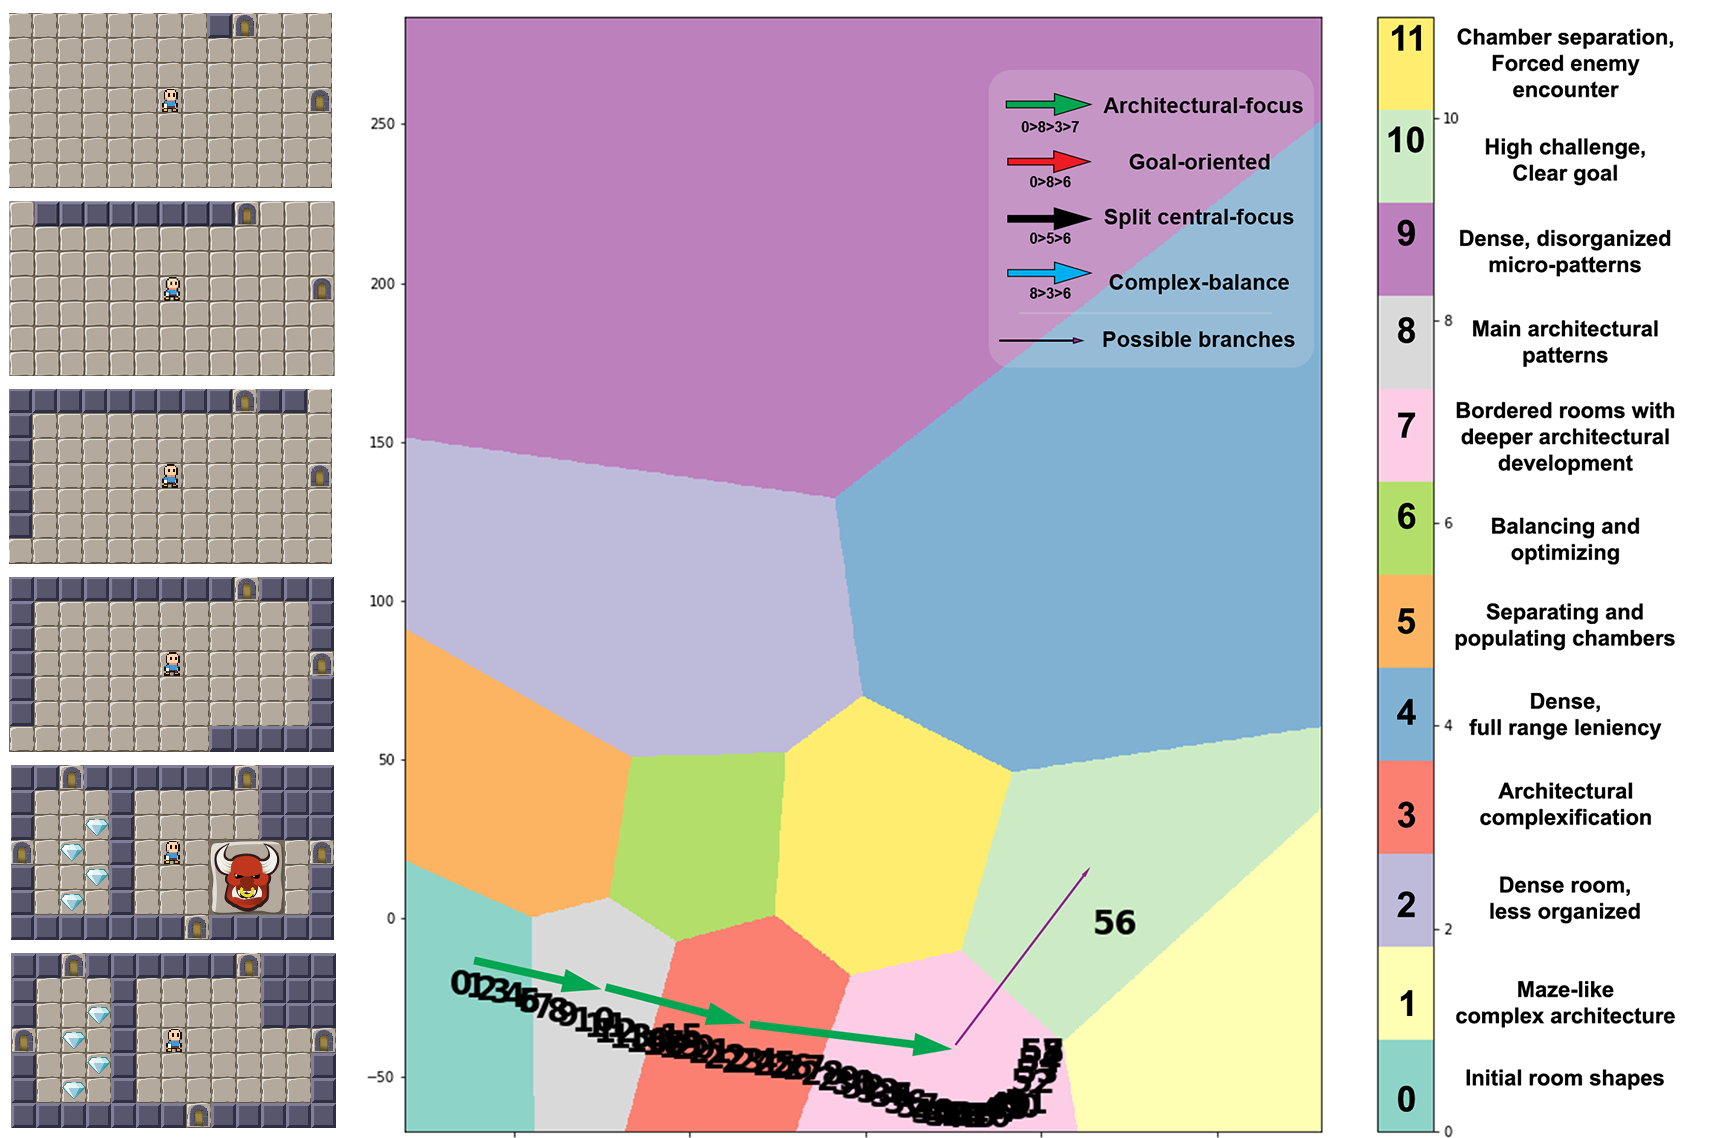
\includegraphics[width=0.45\textwidth]{figures/1.png}
     }
     \hfill
     \subfloat[\textsc{Goal-oriented}\label{p6subfig-2:dummy}]{%
       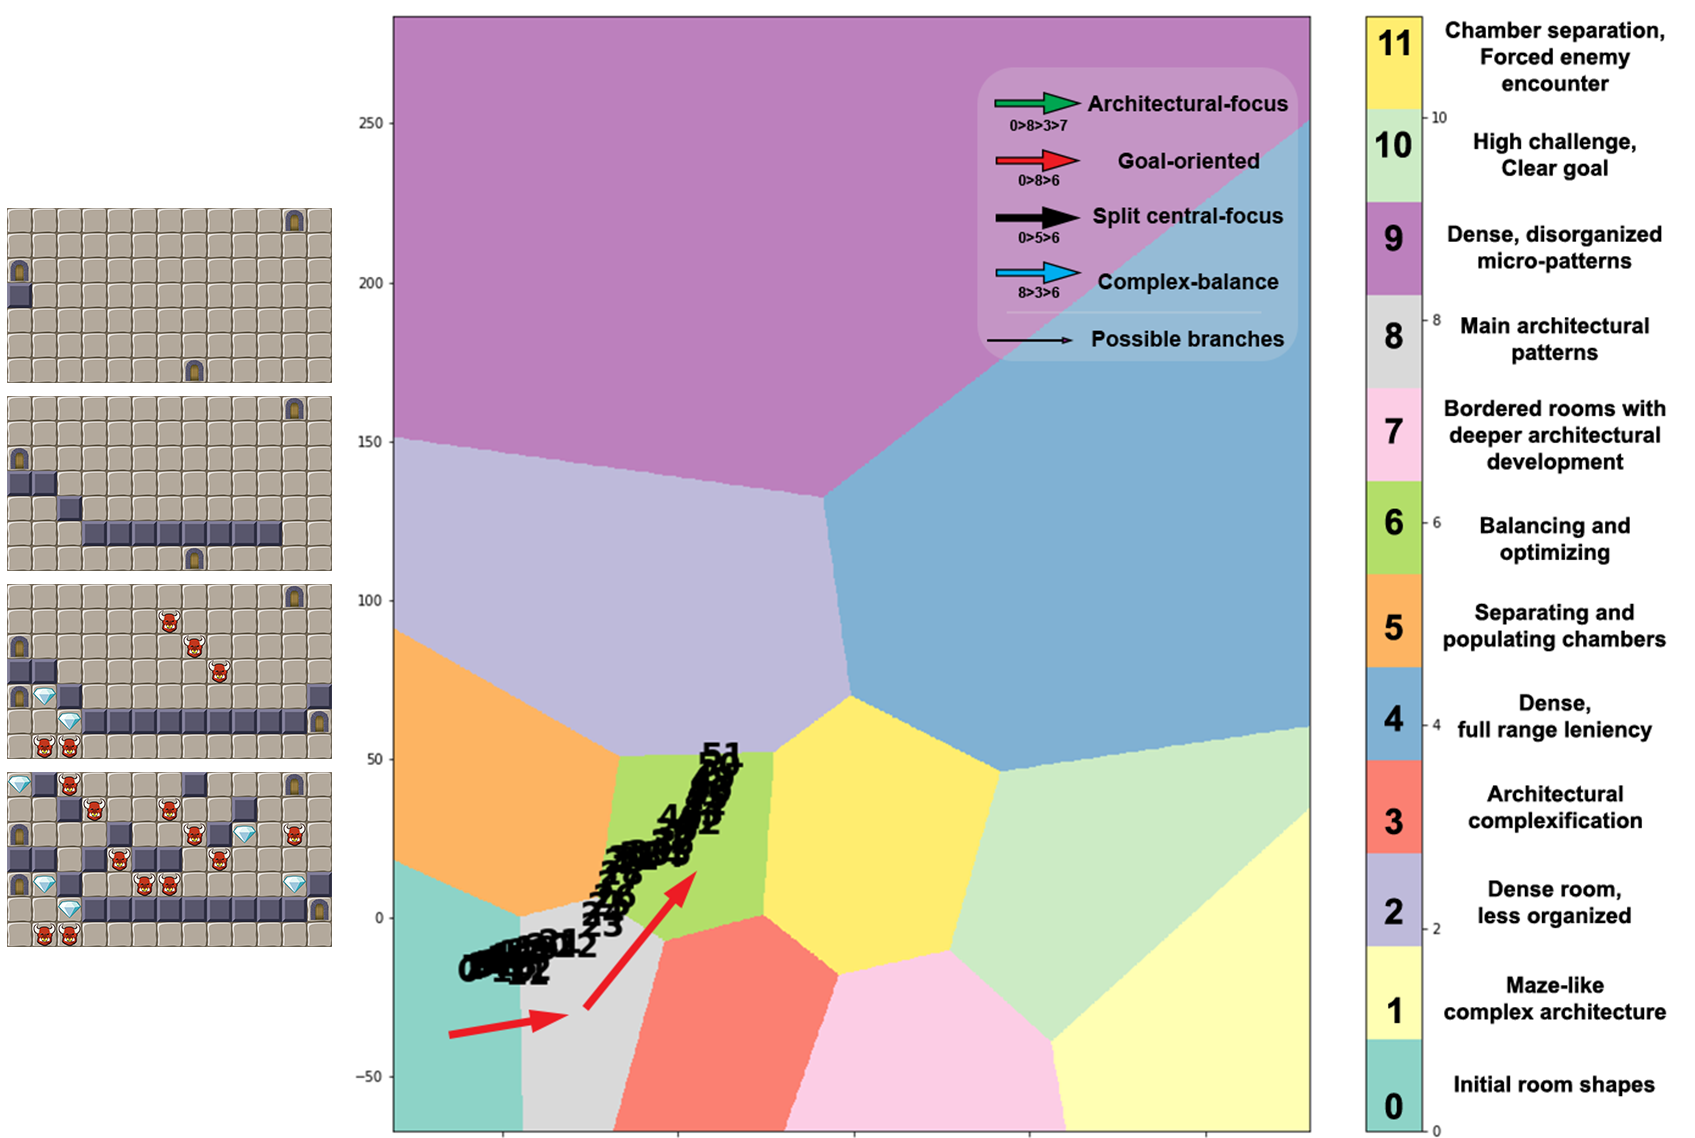
\includegraphics[width=0.45\textwidth]{figures/2.png}
     }\hfill
    %  \medskip
     \subfloat[\textsc{Split central-focus}\label{p6subfig-3:dummy}]{%
       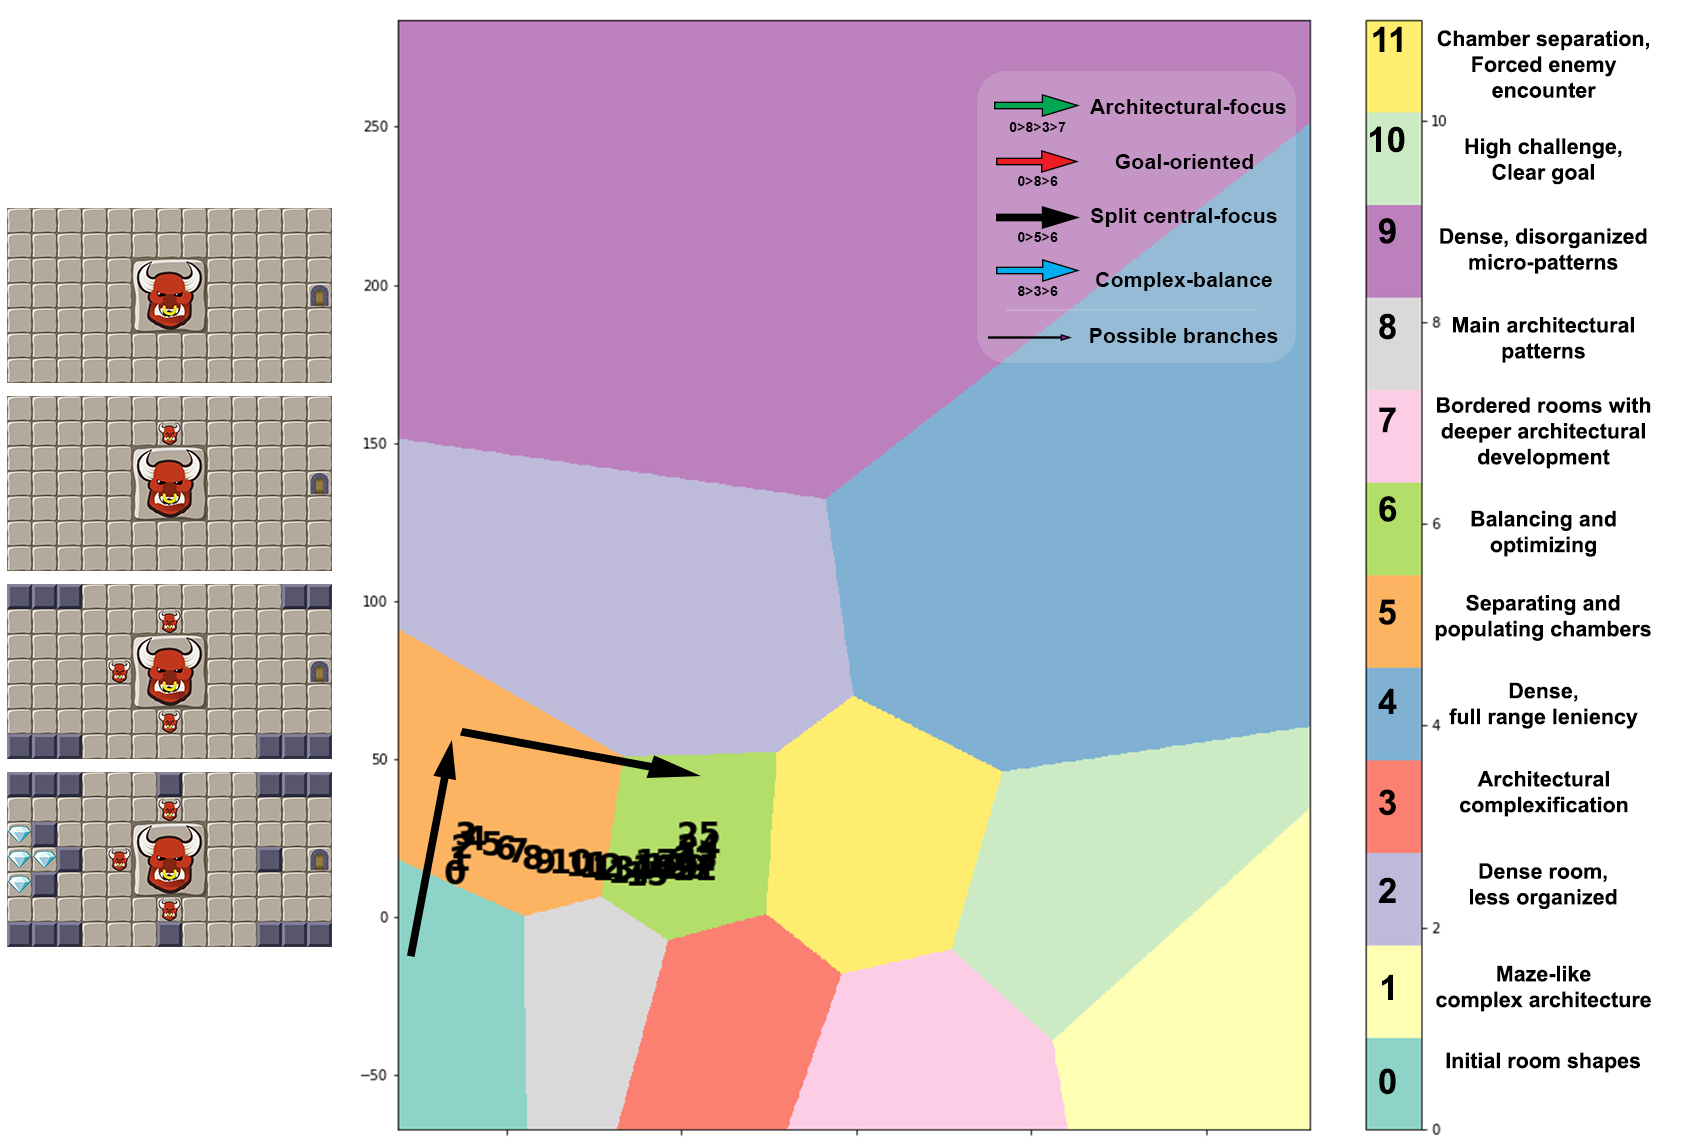
\includegraphics[width=0.45\textwidth]{figures/3.png}
     }
     \hfill
     \subfloat[\textsc{Complex-balance}\label{p6subfig-4:dummy}]{%
       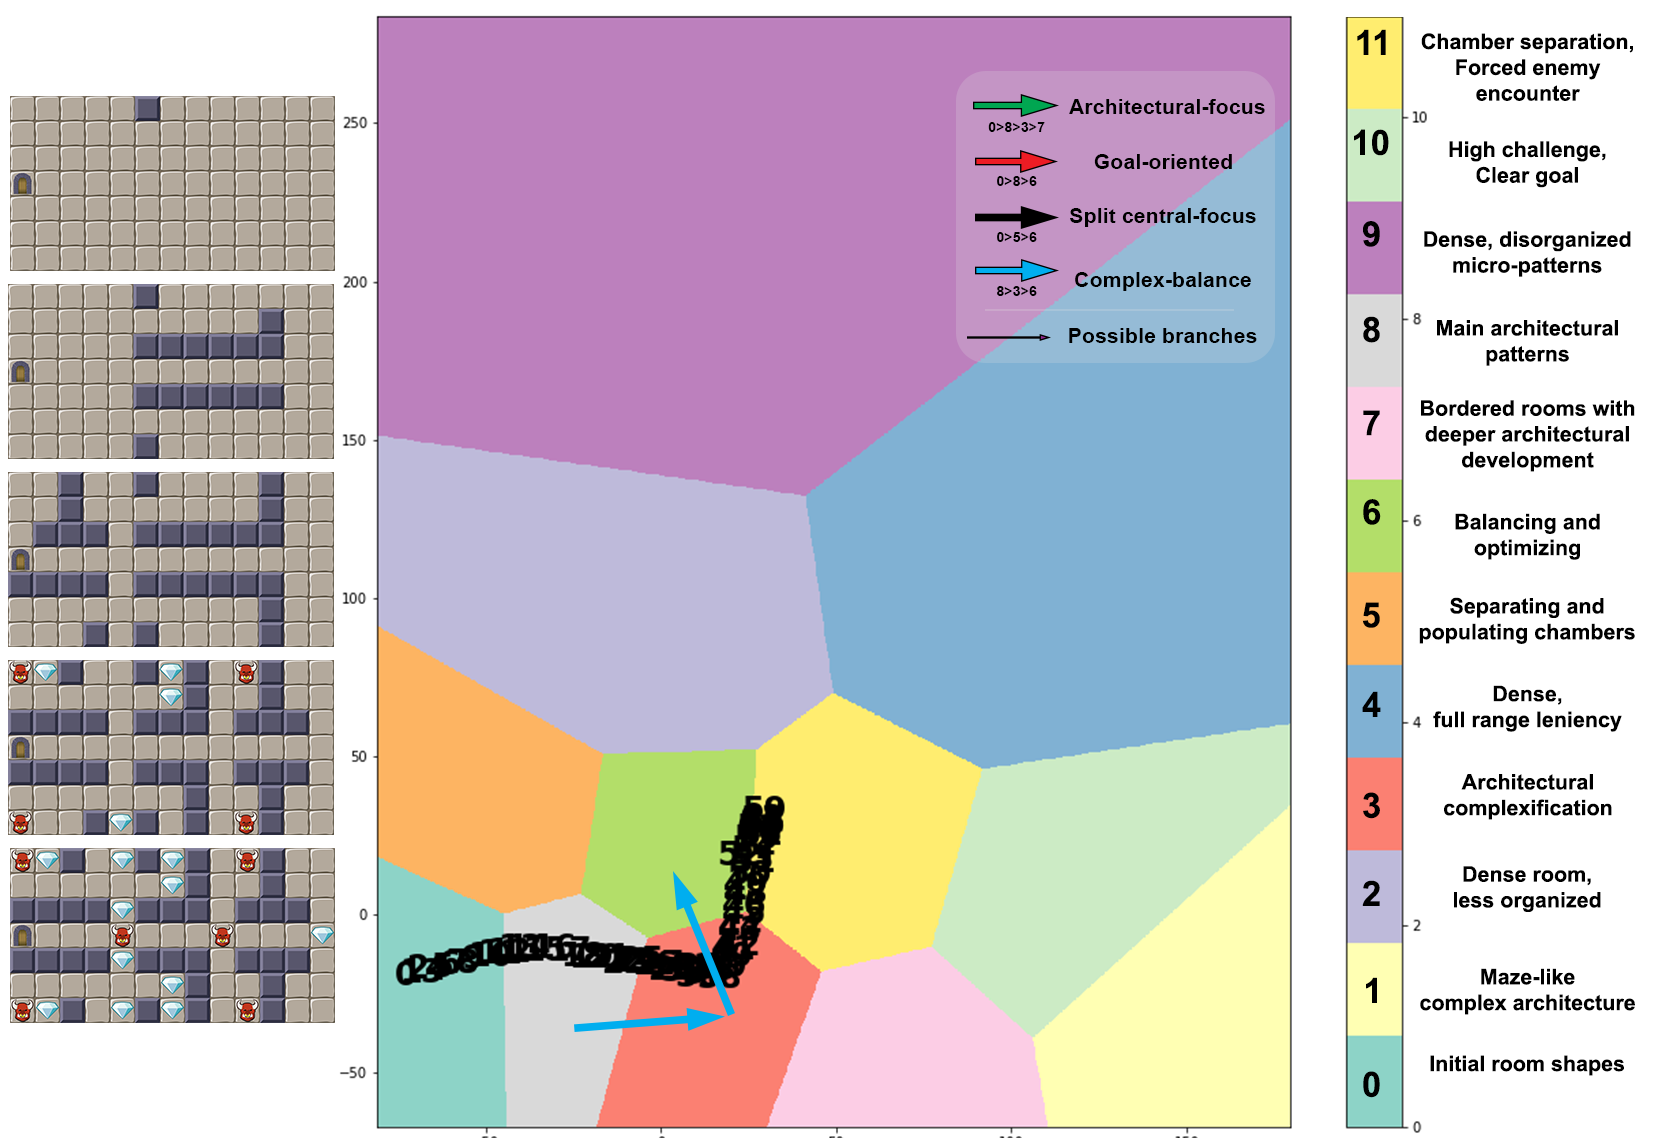
\includegraphics[width=0.45\textwidth]{figures/4.png}
     }
    
    \caption{Examples of each of the archetypical paths from one of the frequent sequences used to create the clusters. To the left of each subfigure, we present each key step in the trajectory i.e. when the design entered a new cluster. (a) presents the \textsc{Architectural-focus} archetypical path where the focus is firstly on creating the structural design of the rooms; the design process jumps back and forth suddenly to cluster 10 (one of the possible branches) due to the designer adding a boss, and removing it immediately. (b) presents the \textsc{Goal-oriented} archetypical path where the design focus on a minimal structure complexity and mix between adding structural changes and enemies/treasures. (c) shows the \textsc{Split central-focus} archetypical path where, intentionally, the designer creates a center obstacle with a boss and build around it. Finally, (d) presents the \textsc{Complex-balance} archetypical path; the design focuses on building complex, uncommon structures first and then add some goal to it with enemies and treasures, taking advantage of the spaces.}
    \label{p6fig:archetypical-examples}
\end{figure*}


Once we created, evaluated, and labeled the clusters, we were able to cluster and visualize the paths of a typical design session. Figure \ref{p6fig:paths-designers} presents an example of the design sessions, where we cluster each step of the design. This sequential process revealed that there is an interesting continuity between clusters, even capturing when a designer probably applied one of the procedural suggestions due to bigger steps in the design style clusters. Further, through this process, we could understand the progress of designers in their design process and represent their trajectory in relation to the traversed clusters rather than individual editions.

\subsubsection{Unique Trajectories}

Using the clusters in Figure \ref{p6fig:all-clusters}, we clustered the design session of all the $180$ designs and collected the unique trajectories that arose from traversing the various clusters. These unique trajectories varied in the starting point, length, and end-point, however, when analyzing the trajectories we identified common patterns among them. They had a similar shape as the following $Unique=$\{0\textgreater8\textgreater4\textgreater7\textgreater10\}, where the first and last element of the sequence are respectively, the starting- and end-points, with all the unique intermediate steps in between.

To gather the common patterns from the trajectories, we applied the Generalized Sequential Pattern (GSP) algorithm, which locates frequent subsequences in the analyzed trajectories. For instance, given three trajectories (a) \{5\textgreater1\textgreater3\textgreater11\textgreater9\}, (b) \{5\textgreater1\textgreater3\textgreater11\textgreater4\, and (c) \{0\textgreater1\textgreater3\textgreater11\}, none of these is a perfect match in its entirety, but GSP can spot that subsequences \{1\textgreater3\textgreater11\}, \{1\textgreater3\}, \{3\textgreater11\}, among others, appear with frequency $= 3$.

%(2) obtain only 1 pattern ($\{5>1>3>11\}$) with frequency=2, if searching from starting points. Finally, using GSP, we find $\{5>1>3>11\}$, $\{1>3>11\}$, $\{1>3\}$, $\{3>11\}$

%We collected these unique trajectories, and 
Furthermore, after doing a preliminary analysis, we identified some steps that we classified as ``border designs'': steps that are borderline between two clusters. These \textit{border designs} disrupted the sequence pattern mining by creating noise in the unique trajectories, specifically when these \textit{border designs} entered a different cluster for just a few steps. %we categorize them as when these "unique" noisy steps were brief.
Therefore, we filtered them out by applying a threshold $\theta = 3$, so that all subsequences inside one cluster with less than $\theta$ steps are removed from the main sequence. I.e, the sample trajectory \{0\textgreater0\textgreater0\textgreater0\textgreater8\textgreater8\textgreater8\textgreater6\textgreater8\} turns into \{0\textgreater8\} instead of \{0\textgreater8\textgreater6\textgreater8\}. Through this, we were able to reduce the noise and the search space, obtaining more meaningful and frequent patterns.

\subsubsection{Archetypical Paths through Style Space}

%Figure \ref{p6fig:finalPaths} shows the archetypical paths taken by designers when creating rooms. Represented as arrows to denote direction, 

%From all the collected unique trajectories, we identified 4 main archetypical paths, which are the ones taken most frequently by designers either as their full path or as the initial path. In Figure \ref{p6fig:finalPaths}, it is shown the archetypical paths, represented as thicker arrows to denote direction, that represent the taken by designers when creating rooms. 

In Figure \ref{p6fig:finalPaths}, we present the archetypical paths, represented as thicker arrows to denote direction, which show the most frequent paths taken by designers either through their whole design process or as the initial meaningful steps. From all the collected unique trajectories, we have identified 4 main archetypical paths, labelled, \textsc{Architectural-focus}, \textsc{Goal-oriented}, \textsc{Split central-focus}, and \textsc{Complex-balance}. In addition, we have numbered each cluster for easier visualization and referencing. 

Moreover, in the figure, it can also be observed thinner purple arrows pointing to different clusters from several of the clusters that are part of the main paths. These are \textit{possible branches} presented in the unique trajectories and added based on their frequency. Through these possible branches, the design of an archetypical session, can vary and extended or deviate the final design. Each archetypical path is defined and explained as follows: 

\paragraph{Architectural-focus}The path followed by this archetype focuses first on designing the architecture of the room with walls. Through this, the design focuses on shaping the visual patterns, chambers, and corridors to give a clear space for adding goals and objectives with enemies and treasures. The sequence is denoted with a green arrow in Figure \ref{p6fig:finalPaths}, and following the sequence \{0\textgreater8\textgreater3\textgreater7\}.

\paragraph{Goal-oriented}Design processes following this archetypical path, create the rooms in a more standard way, combining simpler symmetric wall structures with distributed placement of enemies and treasures. Thus, rather than focusing extensively on an individual part of the room, the rooms have an initial structure and then they are populated with some specific goal-in-mind. The sequence is denoted with a red arrow in Figure \ref{p6fig:finalPaths}, and following the sequence \{0\textgreater8\textgreater6\}.

%Thus, rather than focusing on an individual part of the room until satisfied, the rooms have some initial structures that are populated and continue through an iterative process between these steps.% rooms go through an iterative process of adding have some initial structures that are

\paragraph{Split central-focus}This archetypical path focuses on designing rooms with obstacles placed in the center of the room in the shape of enemies, treasures, or wall structures that clearly split the room into different areas. The design process is less organized than the other archetypes since it searches to achieve the split goal with any of the available tiles. The sequence is denoted with a black arrow in Figure \ref{p6fig:finalPaths}, and following the sequence \{0\textgreater5\textgreater6\}.
%, since the middle step is cluster 5 ("Separating and populating chambers"), which relates to rooms which are expected since the cluster 5 ("Separating and populating chambers") relate to rooms that  as specific structural shapes are not necessary. 

\paragraph{Complex-balance}This archetypical path focuses on building complex symmetric shapes with a clear objective for the player and adapting the spaces with a balance of enemies and treasures. In general, the rooms created following this path are more unique and typically balanced. %   with that adapt well. The process is quite 
The sequence is denoted with a blue arrow in Figure \ref{p6fig:finalPaths}, and following the sequence \{8\textgreater3\textgreater6\}.

Furthermore, using these archetypical paths, we can then categorize certain clusters as key clusters or being more relevant than others based on their contribution to the paths, their frequency, and their usage. Most of the paths go through or end in cluster 6 (``Balancing and optimizing'') and cluster 8 (``Main architectural patterns''), which relate to rooms that have a more explicit mix between corridors and small chambers and more clear architecture. The rooms in those clusters are or shaped as end rooms, as in the case of cluster 6, or architecturally shaped to be “optimized” to a specific goal e.g. a dense bordered room. Similarly, most of the sequences start from cluster 0 ("Initial room shapes"), with $134$ out of the $180$ designs, which correlates to the type of designs encountered in that clusters. Thus, it is understandable that most of the archetypical paths pass through any of these three clusters. 

Nevertheless, it is the steps in-between what creates a clear differentiation between the archetypical paths, which is the benefit of observing the design process as a whole in the clustered room style space. For instance, in fig.~\ref{p6fig:finalPaths}, it can be observed that \textsc{Split central-focus} starts in the same cluster as three other paths, and tentatively ends in the same cluster as three other. However, the designs following \textsc{Split central-focus} are more different to the other trajectories, since it enters a cluster that is denser with several tile types in principle, and where designers seem to have a clearer goal.
% With this, we can further understand why \textsc{Split central-focus} is more different to the other trajectories, since it enters a cluster that is "less organized" in principle. 

%Furthermore, we can also observe that certain clusters are key steps for most paths because they are or a frequent starting or ending point. Most of the paths go through or end in cluster 6 ("Balancing and optimizing") and cluster 8 ("Main structural patterns"), which relate to rooms that have a more explicit mix between corridors and small chambers and a more clear structure, thus, it is understandable since the rooms in those clusters are or shaped as end rooms, as in the case of cluster 6, or structurally shaped to be “optimized” to a specific goal (E.g. dense bordered room, maze-like, more challenging, etc.). However, the distribution of endpoints is quite even, and meanwhile, cluster 6 and cluster 11 ("Chamber separation, Forced enemy encounter") are the most frequent ending points with $36$ and $25$ out of $180$ design processes, the rest of clusters are quite close.

%Similarly, most of the sequences start from cluster 0 ("Initial room shapes"), with $134$ out of the $180$ designs, which correlates to the type of designs encountered in those clusters.

Moreover, in figure~\ref{p6fig:archetypical-examples}, we present examples of each of the designer personas by visualizing the sequence of steps done in representative design sessions, showing how these paths would look like in practice. Each visualization of a designer persona has the key design steps to the left, where each image is in a sequence: the first is the first edition of the designer, the last is the final edition, and the in-between represent entering a new room style cluster. 

In (a), it is shown the \textsc{Architectural-focus}, where the designer first created the border of the room with a clear chamber division. As the designer adds and subsequently removes the boss, the design jumps to cluster 10, which is one of the possible branches, adding a high challenge. In (b), it is shown the \textsc{Goal-Oriented}, where the designer sketched the main shape of the room followed by alternating between enemies, treasures, and walls to design the goal of the player within the room. In this example, the designer ends the design close to cluster 9, with a disorganized placement of tiles and a less aesthetical room, but forming small choke areas balancing the placement of enemies and treasures.

In (c), it is shown the \textsc{Split Central-focus}, where the designer directly started by adding a boss in the center of the room and using this as a reference point, shaped the rest of the room. In (d), it is shown the \textsc{Complex-balance}, where the designer focused on creating an uncommon structure and followed by adding enemies and treasures symmetrically, with clear individual areas for the player to approach.

% It is not surprising to focus on the center as it 

Finally, further analyzing figure~\ref{p6fig:archetypical-examples}, it can also be observed an interesting dual tendency of the designers in the archetypical paths. This dual tendency is to either focus on the aesthetic configuration of the room based on what is perceived in the editor exemplified the personas: \textsc{Architectural-focus} and \textsc{Split central-focus}, and to focus on the player experience exemplified the personas: \textsc{Goal-oriented} and \textsc{Complex-balance}. Nevertheless, both are not mutually exclusive, instead this illustrates adequately the dualistic role the designer has when using the tool and designing rooms. That of creating an aesthetically pleasing object as it is seen in the editor, and that of creating an experience.% However, this is not mutually exclusive. Instead, it shows 


% Furthermore, when analyzing how the different design sequences were clustered and forming the designer personas, we observed an interesting dual tendency of the designers. This dual tendency is to either focus on the aesthetic configuration of the room based on what is perceived in the editor through the personas: \textsc{Architectural-focus} and \textsc{Split central-focus}, and to focus on the player experience through the personas: \textsc{Goal-oriendted} and \textsc{Complex-balance}. This exemplified quite good 
% dualistic role 
% When forming the designer personas, and analyzing how different design sequences


%where the designer focused on creating the shape of the room before adding any enemyfirst created the border of the room

% Finally, in Figure \ref{p6fig:archetypical-examples}, we present examples of each of the archetypical paths to show how would these paths look like in practice, further supporting our findings and path definitions. 

% The archtypical paths a dual tendency of the designers to either go for a strategy that reflects their perception of the level from the editor - like the aesthetic configurations of it, instead of the experiential ones. for example the ones that had a split central focus and a structural focus (which btw maybe i would change to architectural focus). and then there's the ones that have a focus on the player experience like the goal oriented and complex behavior ones. i think this split reflex a very nice dualistic role that the designer has in front of the editor - that of creating an aesthetically pleasing object, as they see it in the editor, and that of creating an experience.
% , and exmplified
%That build around



% Notice that not all the clusters have connectionthat based on the unique trajectories, where designers decided to move towards other areas. 

%it is shown the archetypical paths, represented as thicker arrows to denote direction, that represent the taken by designers when creating rooms. 
% moving from 6 to 11 or from 3 to 11 is a fairly frequent step, thus making it and cluster 6, key points.
% In fact, ending the design at 7 is not that common, thus, 



% the red cluster with $95$ out of the $180$, and from the purple cluster with $49$ out of the $180$, which correlates to the type of designs encountered in those clusters, mainly emptier rooms with initial sketches and shapes. 

% Most of the paths start in cluster 0 ("Initial room shapes") 

% From the figure, we can extract the following clusters as key steps for most of the patterns: "light green", "light blue", "red", and "purple". 

% It can be observed that most of the paths end or go through the "light green" and "light blue" clusters. Both relate to rooms that have a more clear structural pattern and more explicit mix between corridors and small chambers, thus, is understandable since the rooms in those clusters are or shaped as end rooms or structurally shaped to be “optimized” to a specific goal (E.g. dense bordered room, maze-like, more challenging, etc.). Quantitatively, most of the sequences end up in those clusters, $64$ out of the $180$ end in cluster 6 (light blue) and $52$ out of the $180$ end in cluster 11 (light green).


% Similarly, most of the sequences start from the red cluster with $95$ out of the $180$, and from the purple cluster with $49$ out of the $180$, which correlates to the type of designs encountered in those clusters, mainly emptier rooms with initial sketches and shapes. 


% \begin{figure*}
% \centerline{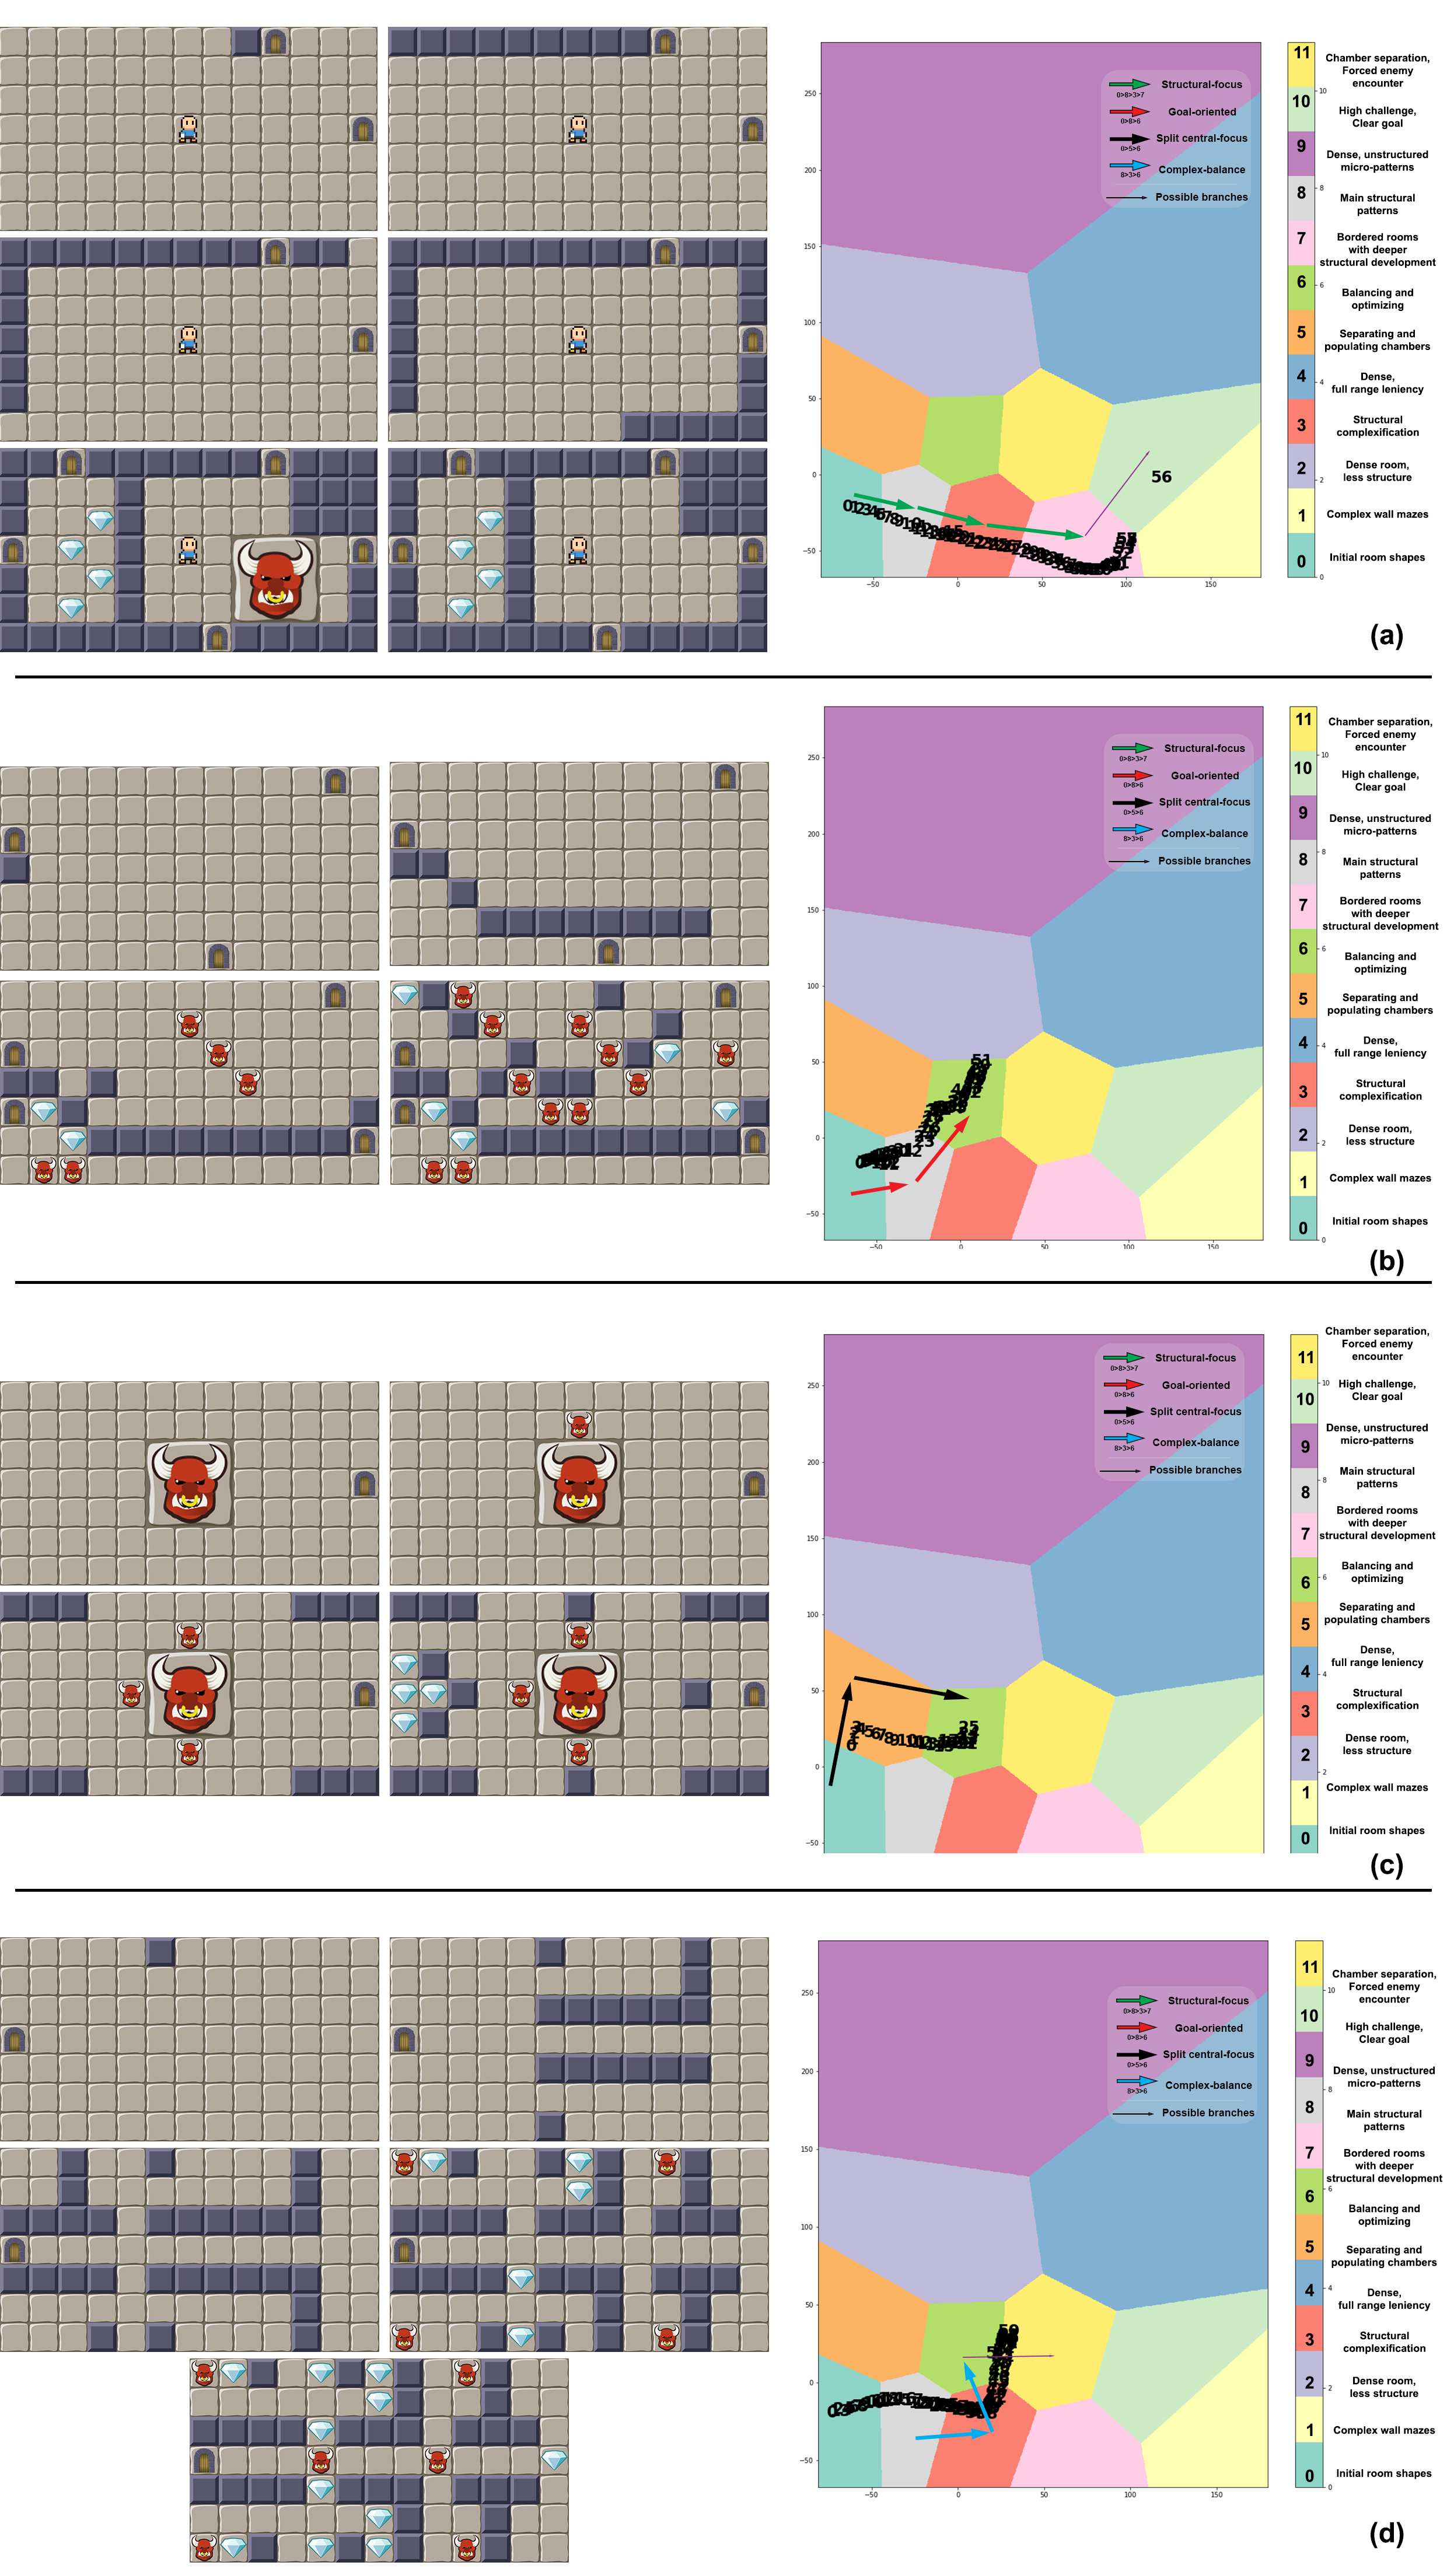
\includegraphics[width=0.7\textwidth]{figures/path-examples-2.png}}
% \caption{Examples of each of the archetypical paths from one of the frequent sequences used to create the clusters. To the left of each subfigure, we present each key step in the trajectory i.e. when the design entered a new cluster. (a) presents the \textsc{Structural focus} archetypical path where the focus is firstly on creating the structural design of the rooms; the design process jumps back and forth suddenly to cluster 10 (one of the possible branches) due to the designer adding a boss, and removing it immediately. (b) presents the \textsc{Goal-oriented} archetypical path where the design focus on a minimal structure complexity and mix between adding structural changes and enemies/treasures. (c) shows the \textsc{Split central-focus} archetypical path where intentionally, the designer creates a center obstacle with a boss and build around it. Finally, (d) presents the \textsc{Complex-balance} archetypical path; the design focuses on building complex uncommon structures first and then add some goal to it with enemies and treasures, taking advantage of the spaces.} \label{p6fig:archetypical-examples}
% \end{figure*}



% \begin{subfigure}[t]{0.33\textwidth}
%         \centering
%         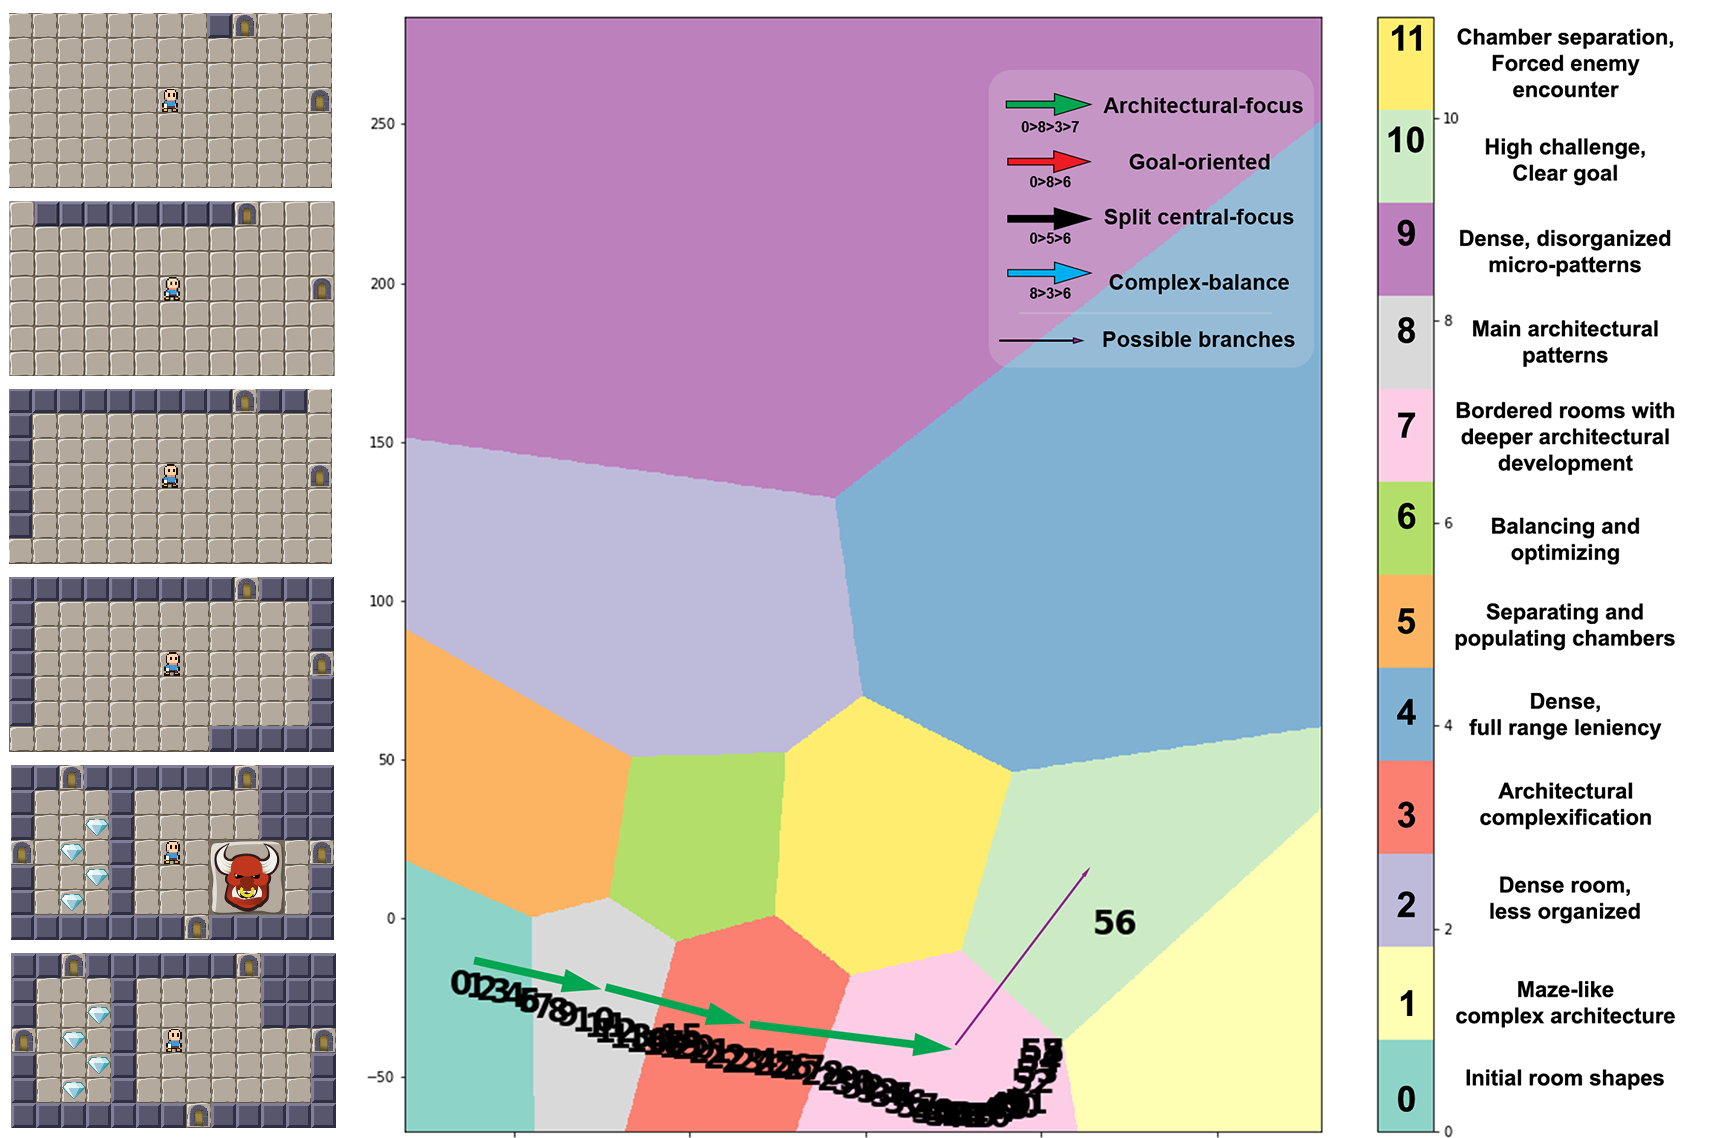
\includegraphics[width=0.95\textwidth]{figures/1.png}
%         \caption{Linearity-\#MesoPatterns}
%     \end{subfigure}%
%     \begin{subfigure}[t]{0.33\textwidth}
%         \centering
%         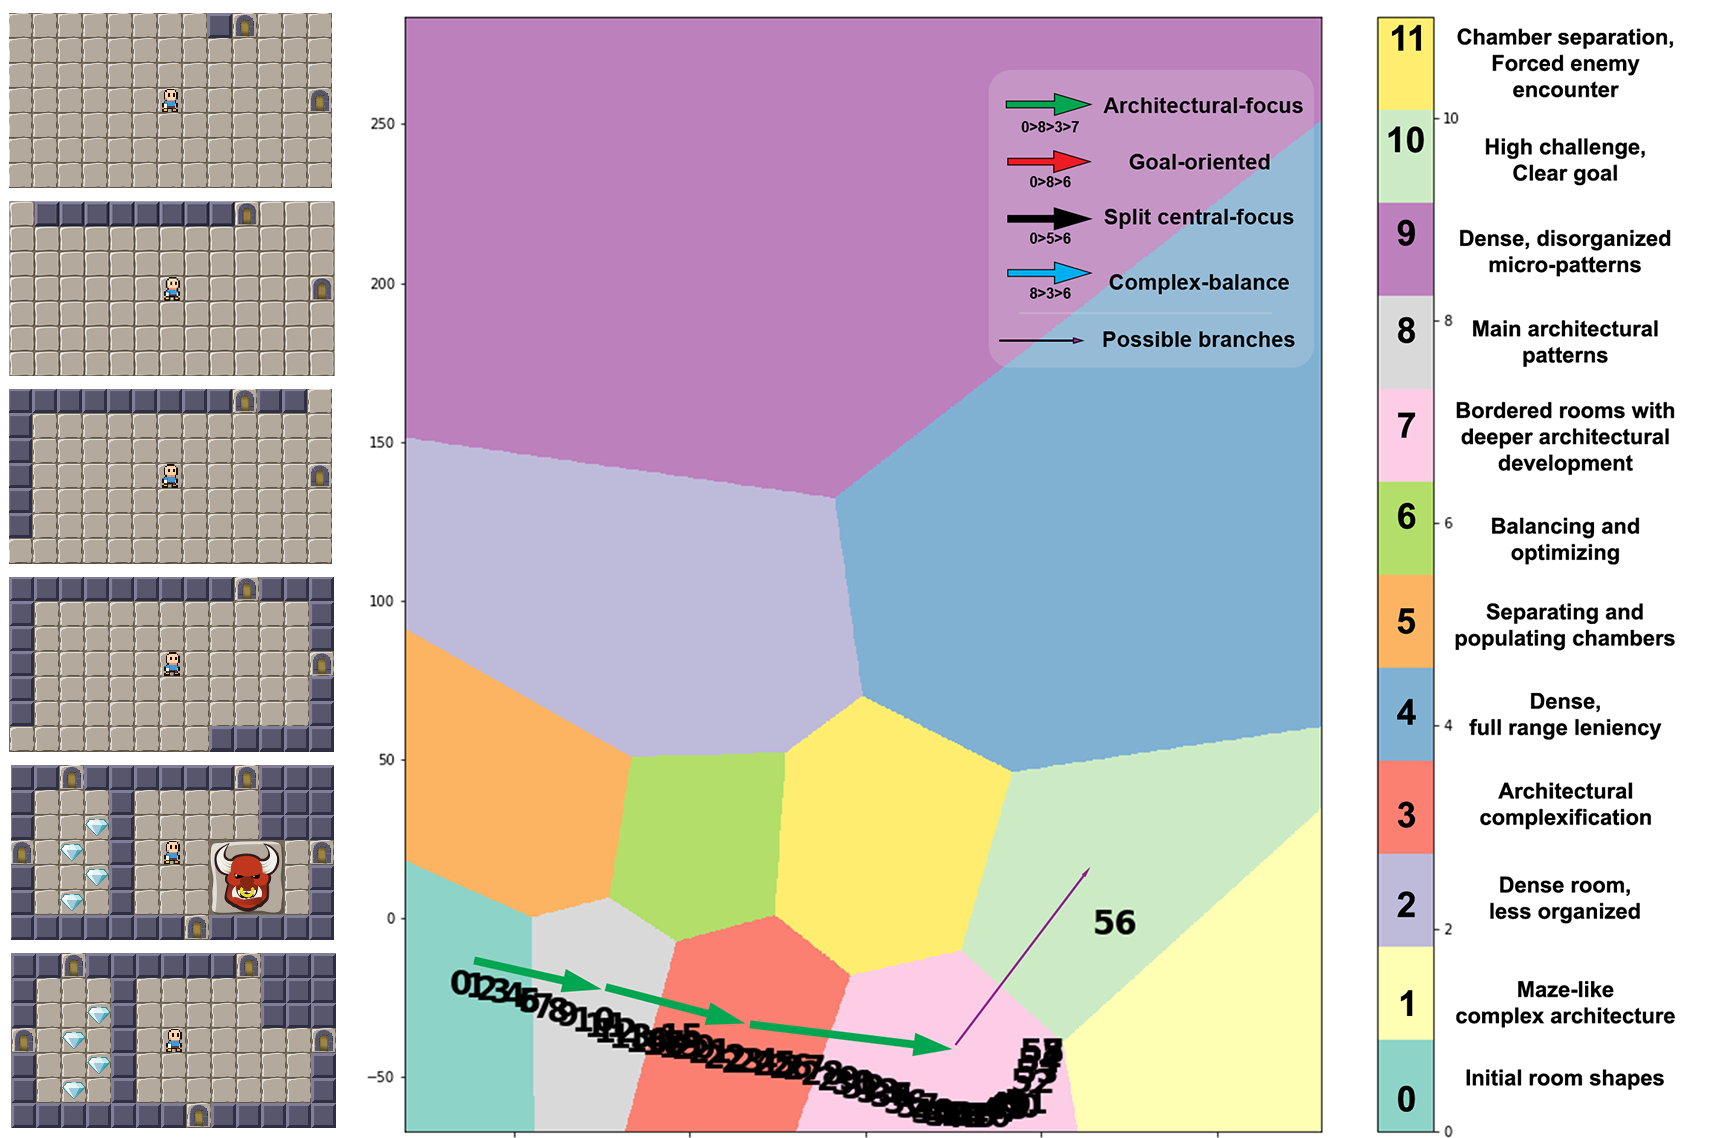
\includegraphics[width=0.95\textwidth]{figures/1.png}
%         \caption{Linearity-\#MesoPatterns}
%     \end{subfigure}%
%     \begin{subfigure}[t]{0.33\textwidth}
%         \centering
%         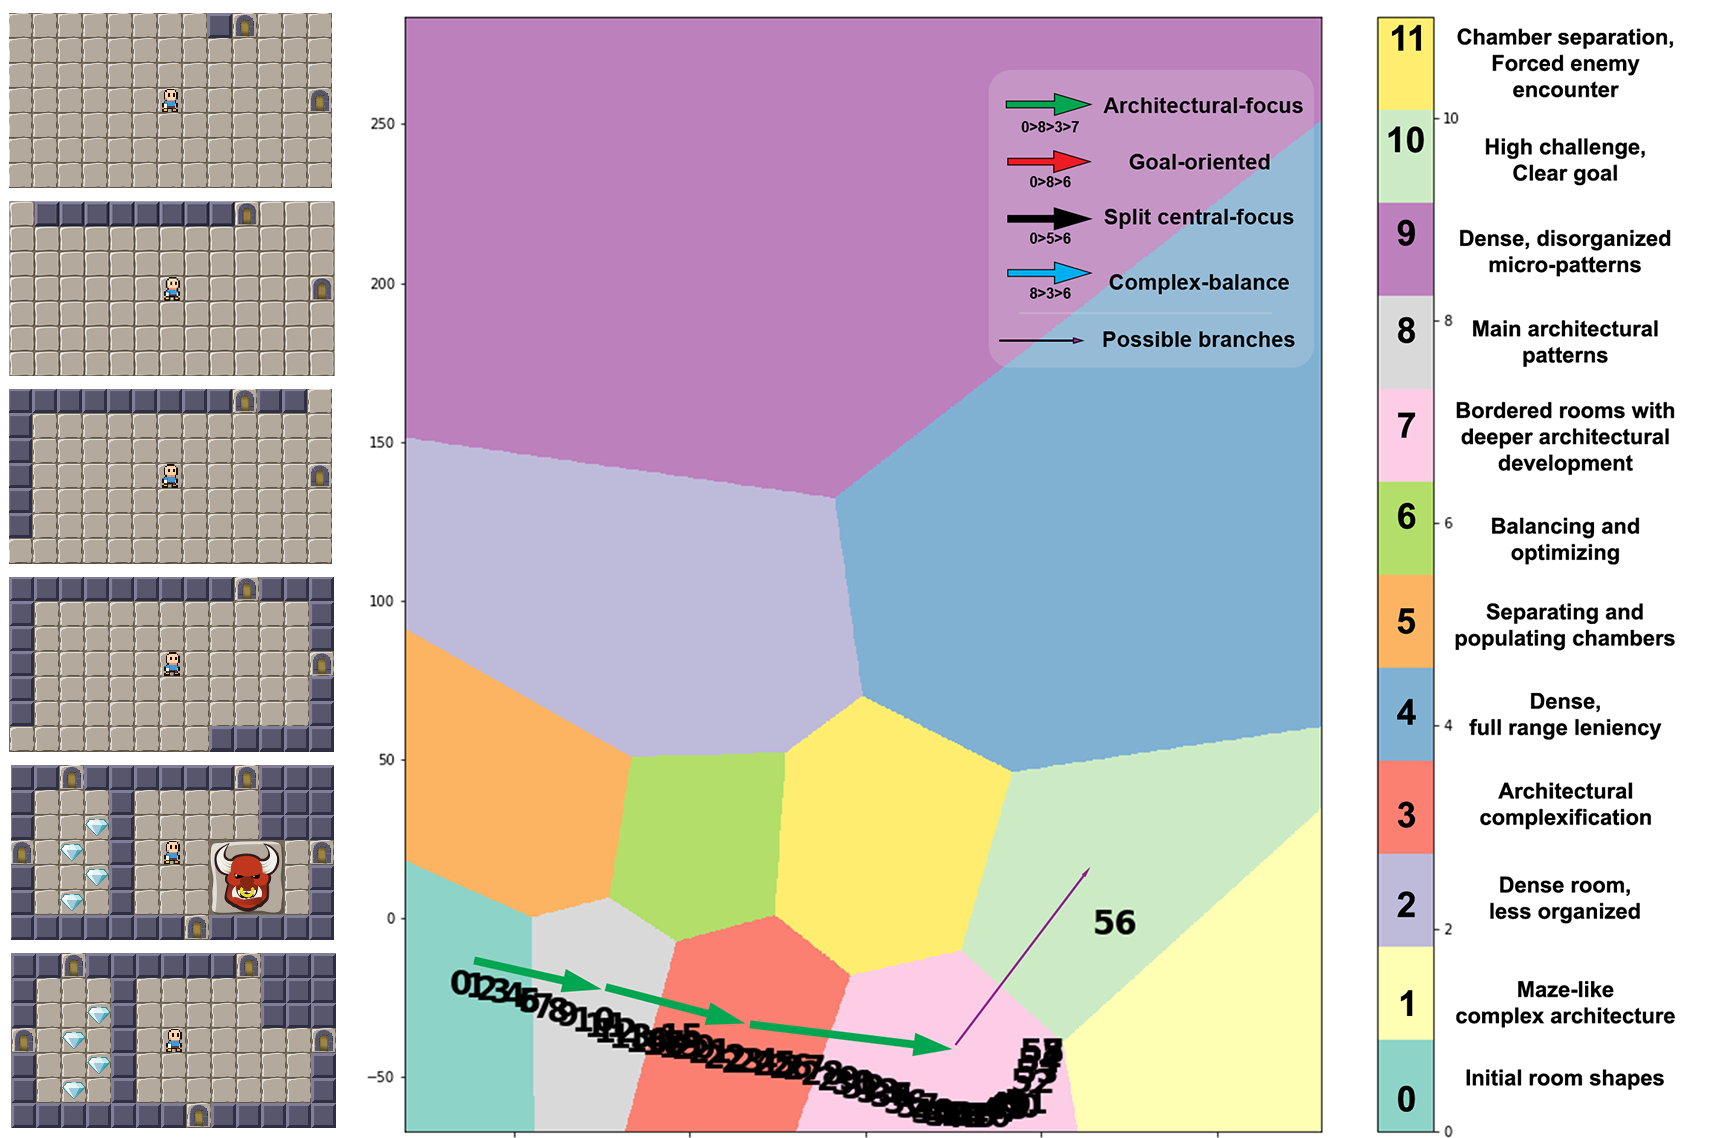
\includegraphics[width=0.95\textwidth]{figures/1.png}
%         \caption{Linearity-\#MesoPatterns}
%     \end{subfigure}%
%     \begin{subfigure}[t]{0.33\textwidth}
%         \centering
%         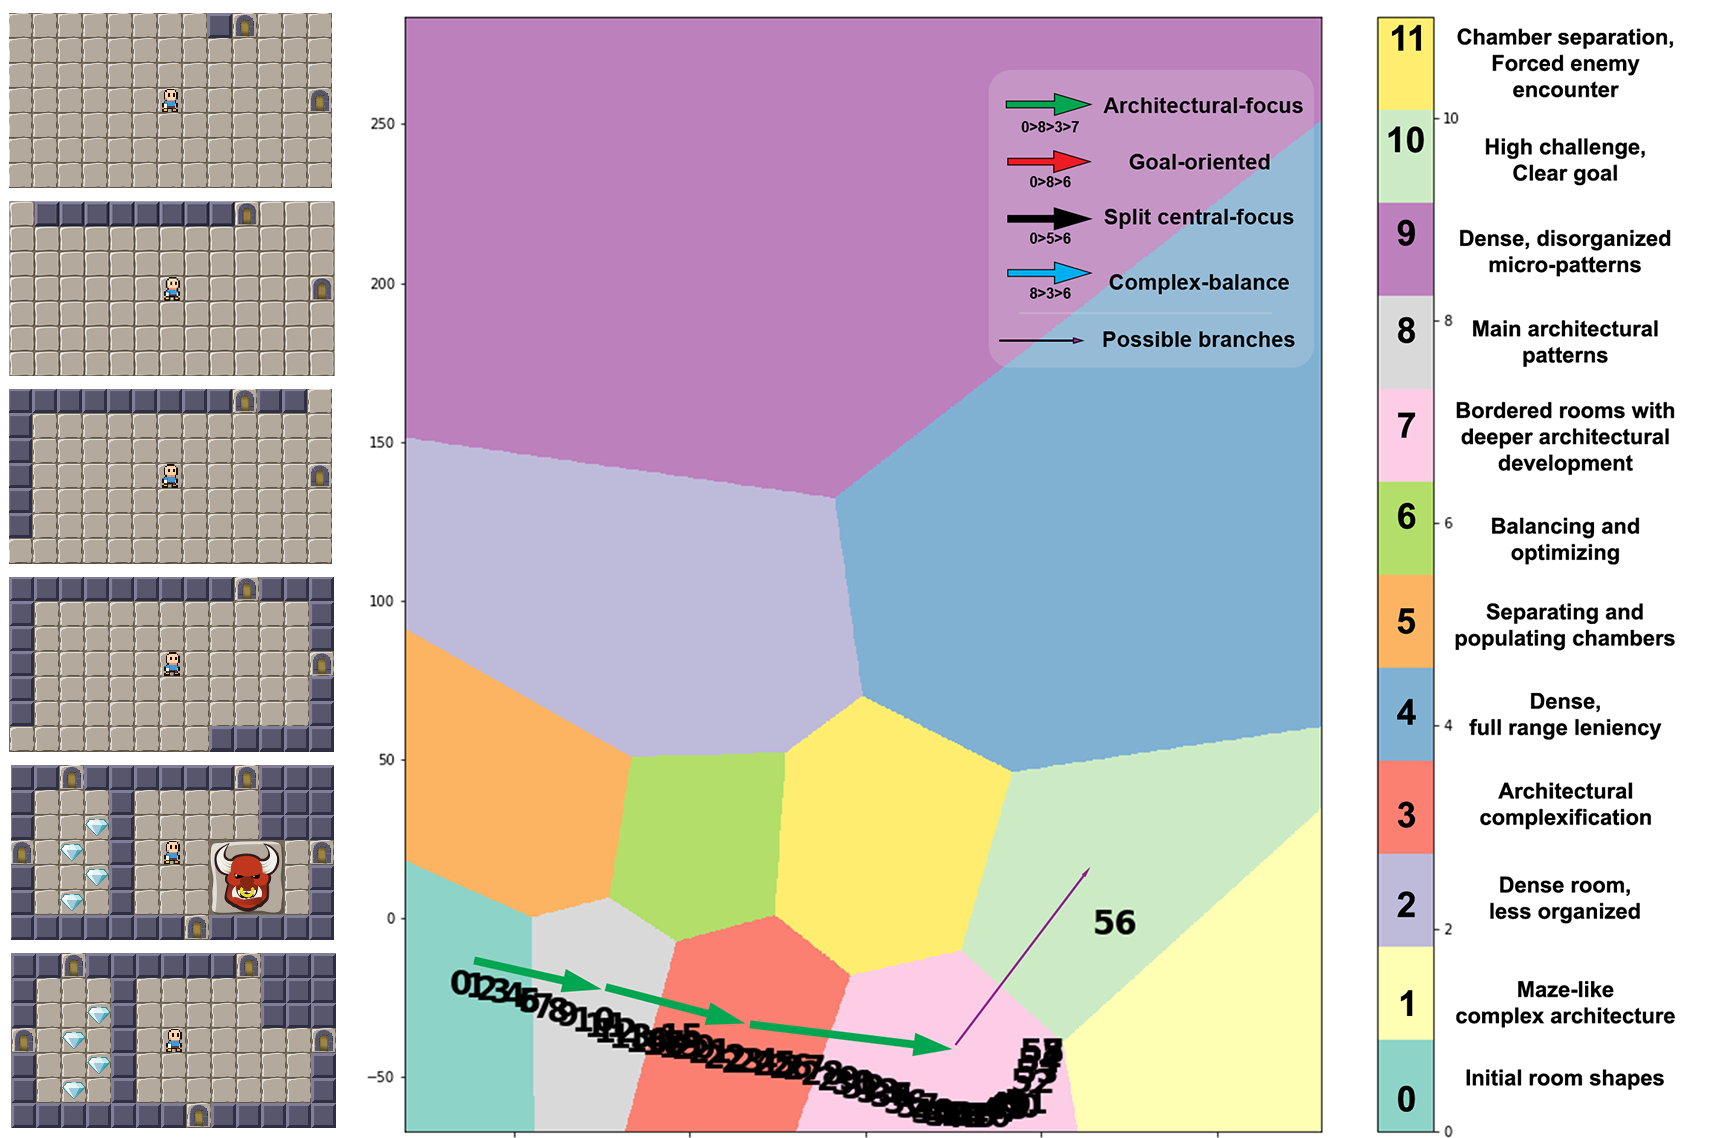
\includegraphics[width=0.95\textwidth]{figures/1.png}
%         \caption{Linearity-\#MesoPatterns}
%     \end{subfigure}%

%From the figure, it can be observed that most of the paths end or go through the "light green" and "light blue" clusters. Both relate to rooms that have a more clear structural pattern and more explicit mix between corridors and small chambers, thus, is understandable since the rooms in those clusters are or shaped as end rooms or structurally shaped to be “optimized” to a specific goal (E.g. dense bordered room, maze-like, more challenging, etc.). Further, most of the sequences end up


%Most of the rooms end there, 64 end in cluster 6 (light blue) and 52 end in cluster 11 (light green), so it makes sense that they are key steps in most of the subsequences. Further, most of the rooms start in cluster 0 (red) – 95 rooms – or in cluster 8 (purple) – 49 rooms, which make them key steps as well

%Most of the sequences with $95$ out of the $180$ starting in the red cluster, and $49$ out of the $180$ starting in the purple cluster. which correlates to the type of designs encountered in those clusters, mainly emptier rooms with initial sketches and shapes. 


%Info about the trajectories, 1) variation (length), 2) starting cluster, 3) end-point cluster.


% \begin{itemize}
%     \item[\textbf{DONE:}] Present 3 representative examples where we cluster each step of the design process. Perhaps I should create a room that would go through all the clusters?
%     \item[\textbf{DONE:}] Explain that we did this for all the 180 designs, and we collected the unique trajectories along the clusters, reducing the dimensionality of each step to each cluster.
%     \item[\textbf{DONE:}] Due to border designs (step that are in the border between 2 different clusters), we applied a threshold to reduce the noise those inputs could have when clustering the trajectories of the designer.
%     \item[\textbf{DONE:}] this data (the sequences) were then applied the GSP algorithm, a subsequence frequent pattern mining algorithm, to extract the frequent patterns in the sequences (including subsequences within the sequence).
%     \item This resulted in the following trajectories, which can also be observed in Figure X.
%     \item 
% \end{itemize}

\subsection{Conclusions}



% \begin{itemize}
%     \item Discussion on what does this archetypical design trajectories mean?
%     \item how to use them? next steps into integrating this into a system. To use this in a search-based approach as objectives for the generation to move towards the directions where (according to our archetypical design trajectories) the designers will move towards in their design process. Perhaps I could also bring the discussion from the workshop-paper for HC-AI.
%     \item discussion on creativity? is the output or the process where the actual creativity is outputted? Compare using end-design clustering to using sequences to cluster.
%     \item Discussion on how PCGRL relates to this type of work? --> Perhaps this is something for the background instead.
% \end{itemize}{}


% This paper presents a step towards designer modelling in a MI-CC environment by providing an implementation of designer personas as archetypical trajectories through style space, as a means to characterize several representative and frequent design styles together. 

%This paper presents a novel approach and meaningful steps towards designer modeling in an MI-CC environment. By providing an implementation of designer personas as archetypical trajectories through style space, we show that 

This paper presents a novel approach and meaningful steps towards designer modeling through an experiment on archetypical design trajectories analysis in an MI-CC environment. Through this, we characterize several representative design styles as designer personas. We have first run and compared several clustering setups to find the best partitioning of the design style using the edition sequences of the collected $180$ unique rooms, ending in $8196$ data points, and resulting in a set of twelve cohesive, coherent, and meaningful clusters. We have then mapped these $180$ design sequences in terms of these clusters, applying frequent sequence mining to find four frequent and unique designer styles, with related common sub-styles. As a result, we have presented a roadmap of design styles over a map of data-driven design clusters. 

%This paper presents a step towards designer modeling through an experiment on archetypical design trajectories analysis in an MI-CC environment, as a means to characterize several representative design styles as designer personas. We have first run and compared several clustering setups to find the best partitioning using the edition sequences of the collected $180$ unique rooms, ending in $8196$ data points, and resulting in a set of twelve cohesive, coherent, and meaningful clusters. We have then mapped these $180$ design sequences in terms of these clusters, applying frequent sequence mining to find four frequent unique designer styles, with related common sub-styles. As a result, we have presented a roadmap of design styles over a map of data-driven design clusters. %The examples in Figure \ref{p6fig:archetypical-examples}, help us to clarify 

%  namely the \textsc{Designer Personas}

% Our work draws on the ideas, concepts, and goals and concepts proposed by Liapis et al. when introducing the Designer Modeling as a model to capture multiple designer's processes. A prototype of such was implemented in the sentient sketchbook~\citepsixth{p6Liapis2014-designerModelImpl}, where it is proposed the use of interactive evolution by biasing the search space in favor of hand-crafted features of the design. we propose an alternative and novel route to designer modeling through clustering the design space and the room style based on the collected data. Moreover, we differ as well on the type of level design, being the sentient sketchbook a tool for strategy games~\citepsixth{p6liapis_generating_2013}, while EDD a tool for adventure and rogue-like games~\citepsixth{p6Alvarez2020-ICMAPE}. These differences strengthen the importance and usefulness of designer modeling, and highlight the holistic and generic properties of this designer-centric perspective.

Designer modeling was proposed as an approach to capture multiple designer's processes to create a better workflow by Liapis et al.~\citepsixth{p6Liapis2013-designerModel}, and our work draws on many of their ideas, concepts, and goals. Furthermore, a prototype of such was implemented in the sentient sketchbook~\citepsixth{p6Liapis2014-designerModelImpl}, where it is proposed different approaches to model style, process, and goals based on choice-based evolution and the designer's current design to adapt the provided suggestions accordingly. We propose an alternative route to designer modeling through clustering the design space and the room style based on the collected data. Moreover, we differ in the type of level design, being the sentient sketchbook a tool for strategy games~\citepsixth{p6liapis_generating_2013}, while EDD is a tool for adventure and rogue-like games~\citepsixth{p6Alvarez2020-ICMAPE}. These differences strengthen the importance and usefulness of designer modeling and highlight the holistic and generic properties of this designer-centric perspective and its possibilities.

% Designer modeling in computer-aided design tools was proposed by Liapis et al.~\citepsixth{p6Liapis2013-designerModel} as an approach to capture multiple designer's processes to create a better workflow, and a prototype of such was implemented in the sentient sketchbook~\citepsixth{p6Liapis2014-designerModelImpl}. While our work drags on many of the concepts, ideas, and goals described by Liapis et al., we propose an alternative route to designer modeling through clustering the design space

% In their work, they propose the use of hand-crafted

% Our work drags on many of the concepts, ideas, and goals described in~\citepsixth{p6Liapis2013-designerModel}, but we propose an alternative route to designer modeling through clustering the design space and the room style based on the collected data. In contrast 

% Their work propose the use of interactive evolution by biasing the search space in favor of hand-crafted features of the design akin to~\citepsixth{p6Alvarez2020-DesignerPreference}. However, we propose an alternative and novel route to designer modeling through clustering the design space and the room style based on the collected data. Moreover, we differ as well on the type of level design, being the sentient sketchbook a tool for strategy games~\citepsixth{p6liapis_generating_2013}, while EDD a tool for adventure and rogue-like games~\citepsixth{p6Alvarez2020-ICMAPE}. Applying the idea of designer modelling to both genres, not only shows the importance and usefulness of designer modeling but also the holistic and generic view 

% These differences strengthen the importance and usefulness of designer modeling, and highlight the holistic and generic properties of this designer-centric perspective.

% % might be interesting to discuss this.
% While the approach described in this paper is applied in a tool for creating zelda-like dungeon games~\citepsixth{p6tloz}, the approach can be reused and extended to other domains 

These contributions allow us to better understand, cluster, categorize and isolate designer behavior. This is very valuable for mixed-initiative approaches, where a clear virtual model of the designer's style allows us to better drive the search process for procedurally generating content that is valuable for the designer. Designer personas have the potential to be used in many different scenarios. For instance, as objectives for a search-based approach to enable a more style-sensitive system, to evaluate the fitness of evolutionary generated content or to train PCG agents via Reinforcement Learning~\citepsixth{p6khalifa2020-pcgrl}. 

Moreover, recognizing the designers' current style and the path taken so far, which would indicate a possible designer persona, could open the possibility for recognizing their intentions, preferences, and goals. This traced roadmap of designer personas could let a content generator anticipate a designer's next moves without heavy computational cost, just by identifying her current location on the map and offering content suggestions that lie in the most promising clusters to be visited next. Conversely, it could also identify designers who do not follow a certain path, i.e. deviating from the pattern, trying to understand their objective through their design style.

% Finally, in our work, we did not observe any type of cross-path i.e. a design going from one path to another. We believe that this is due to the level at which we observe the archetypical paths. However, preliminary analysis on the dataset used in this paper and as expected, the design process of designed rooms within the same dungeon does follow different paths, and sometimes even crossing each other. This opens an interesting and exciting area to explore a wider layer, taking rooms as a set of archetypical paths taken by designers. Observing the paths taken in previous and future rooms, and the dungeon as a whole, as briefly introduced in section~\ref{p6sec:designStyle}, to understand the designers' intentions and goals when they proceed to create a new room is a promising future step to take with the current system. 

%  i.e. room-wise, as the designer typically would design the room with a set of goals

Finally, it is also important to observe the nature of the previous and future rooms created by a designer. Observing the dungeon as a whole, as briefly introduced in section~\ref{p6sec:designStyle}, to understand the designers' intentions and goals when they proceed to create a new room is a promising future step to take with the current system. 

% Furthermore, the designer personas addresses the dynamic-dynamic system vs. dynamic-static system open question raised by Alvarez and Font~\citepsixth{p6Alvarez2020-DesignerPreference}, which relates to the challenge of adapting a system to the a ever-changing designer. With the use of the archetypical paths, the model is not anymore adapting and moving through the solution space with the designer, rather the designer traverse through an already clustered space. 

% With the use of the archetypical paths, we can not only identify the current designer persona the designer is following but we can also adapt and anticipate to what they might end up doing. 

% Furthermore, the designer personas addresses an open question raised by Alvarez and Font \citepsixth{p6Alvarez2020-DesignerPreference}, related to the challenges  using a dynamic-dynamic system vs. a dynamic-static system. The authors describe the dynamic-dynamic system as a system where both designer and AI-system move through the solution space, with the AI-system constantly trying to adapt to the designer. They concluded that the main challenge correspond to designers constantly concept drifting resulting in them continuously changing their decisions. Instead, the authors proposed the use of a dynamic-static system, where the model is not anymore adapting and moving through the solution space with the designer, rather the designer traverse through an already clustered space. With the use of the archetypical paths, we can not only identify the current designer persona the designer is following but we can also adapt and anticipate to what they might end up doing. 


%and conclude that the main challenges in

% Moreover, this traced roadmap of designer personas could let a content generator anticipate a designer's next moves without heavy computational cost, just by identifying her current location on the map and offering content suggestions that lie in the most promising clusters to be visited next. %Further, one could also be able to identify designers that do not follow a certain path i.e. deviating from the pattern, and try to understand through their design style their objective.





% From the $180$ unique rooms, we extracted and used the edition sequence of each of the rooms, from their initial design to the more elaborated end-design, to compose a richer dataset that could capture the design process of a designer rather than focusing on the end-point. Through this, we ended up using $8196$ data points in our dataset.

% We have first run and compared s


% through experimenting with 

% This paper presents a step towards designer modelling by providing a prototype implementation of designer personas as archetypical trajectories through style space. These archetypical paths

% This paper presents an experiment on archetypical design trajectories analysis in a MI-CC environment, as a means to characterize several representative design styles as designer personas. We have first run and compared several clustering setups to find the best partitioning, resulting into a set of twelve cohesive, coherent, and meaningful clusters. We have then mapped almost 200 complete design sequences in terms of these clusters, applying sequence mining to find four frequent unique designer styles, with related common sub-styles. As a result, we have presented a roadmap of design styles over a map of data-driven design clusters. 



% be used as goal for other systems were anticipating a design or creating a synthetic objective might be more complicated. We envision that these designer personas can be used within 

\bibliographystylepsixth{ieeetr}
\bibliographypsixth{included-papers-tex/paper-6/references.bib}